
\documentclass[preprint,12pt,authoryear]{elsarticle}
\usepackage[verbose,letterpaper,tmargin=2.54cm,bmargin=2.54cm,l
margin=2.54cm,rmargin=2.54cm]{geometry}

%References can be split up over multiple lines
\usepackage{breakcites}
\usepackage{times}

\usepackage{amsmath}
\usepackage[colorinlistoftodos]{todonotes}
\usepackage[colorlinks=true, allcolors=blue]{hyperref}

\usepackage{hyperref}

%% The graphicx package provides the includegraphics command.
\usepackage{graphicx}
%% The amssymb package provides various useful mathematical symbols

%%Allows text in equations
\usepackage{amssymb}
%%Make sure caption does not stick to the table
\usepackage{caption} \captionsetup[table]{skip=10pt}
%%Multiple rows in complex tables
\usepackage{multirow}

%%Two figures aside
\usepackage{caption}
\usepackage{subcaption}

%%Floatbarrier prevents figures to be above section title 
\usepackage{placeins}

%%Forced line break within cell
\usepackage{makecell}
\renewcommand\theadalign{bc}
\renewcommand\theadfont{\bfseries}
\renewcommand\theadgape{\Gape[4pt]}
\renewcommand\cellgape{\Gape[4pt]}

\usepackage[T1]{fontenc}
\usepackage[utf8]{inputenc}
\usepackage{floatrow}

%Packages for running title
\usepackage{fancyhdr}
\pagestyle{fancy}

%re-scale tables 
\usepackage{graphics}

%% The lineno packages adds line numbers. Start line numbering with
%% \begin{linenumbers}, end it with \end{linenumbers}. Or switch it on
%% for the whole article with \linenumbers after \end{frontmatter}.
\usepackage{lineno}

%% Double space
\usepackage{setspace}

%% Roman letters
\newcommand{\RNum}[1]{\uppercase\expandafter{\romannumeral #1\relax}}

%Acknowledgments
\newcommand{\ackname}{Acknowledgments}

%Authors’ contributions
\newcommand{\autcont}{Authors’ contributions}

%Data accessibility 
\newcommand{\datacc}{Data accessibility}

\usepackage{moreverb} % for verbatim output

% Glossary
\usepackage[utf8]{inputenc}
\usepackage{hyperref}
\usepackage{glossaries}
\usepackage{calc}
\usepackage{booktabs}
\usepackage{tabularx}% (for comparison)

\journal{Ecological Informatics}

% Running title
\rhead{Uncertainty of passive telemetry data}
\lhead{}
\setlength{\marginparwidth}{2cm}

\begin{document}
%double spacing to facilitate the reviewing process
\begin{spacing}{1.9}
%%\begin{flushleft}
\begin{frontmatter}

%% Title, authors and addresses

\title{%
Quantifying and reducing epistemic uncertainty of passive acoustic telemetry data from longitudinal aquatic systems \\
\large }

\author{Stijn Bruneel$^{1,2\ast}$, Pieterjan Verhelst$^{2}$, Jan Reubens$^{3}$, Jan M. Baetens$^{4}$, Johan Coeck$^{5}$, Tom Moens$^{2}$, Peter Goethals$^{1}$}

\address{$^{1}$Department of Animal Sciences and Aquatic Ecology, Ghent University, Coupure Links 653, 9000 Ghent, Belgium,

$^{2}$Marine Biology Research Group, Ghent University, Krijgslaan 281, 9000 Ghent, Belgium,

$^{3}$Flanders Marine Institute (VLIZ), Wandelaarkaai 7, 8400 Ostend, Belgium,

$^{4}$Department of Data Analysis and Mathematical Modelling, Ghent University, Coupure Links 653, 9000 Ghent, Belgium

$^{5}$Research Institute for Nature and Forest (INBO), Havenlaan 88, bus 73, 1000 Brussels, Belgium,

$^\ast$To whom correspondence should be addressed; E-mail: stijn.bruneel@ugent.be}

\begin{abstract}

\linenumbers

Passive acoustic telemetry data are used to study animal movement in aquatic environments, but tools to process the data are limited. In areas that are too large to be fully covered by the limited detection ranges of receivers or acoustic listening stations, researchers generally assume that animals are residing in an area when they are detected frequently at specific receivers. There is, however, no consensus on how this area and frequency should be spatially and temporally defined respectively, thereby introducing some unaccounted uncertainty of this residency-at-receivers. In longitudinal aquatic systems such as rivers or estuaries, strategically placed receivers are often used as gates or curtains through which tagged animals have to pass. Rather than being a proxy for the time spent near receivers, the detections can serve as boundary conditions to delineate the durations that animals spent between receivers (i.e. residency-between-receivers). As such, providing a spatial and temporal context to the detections and enabling the quantification of epistemic uncertainty. To assess the usefulness of this approach, we analyzed telemetry data for migrating eel in a longitudinal estuarine acoustic tracking network of 21 gates. Results revealed a logarithmic relationship between epistemic uncertainty and gate network resolution, which indicates that transferring information from the spatial to the temporal level has a positive effect on the epistemic uncertainty. The poor correlation between the at-receivers and the between-receivers approach indicates that the latter, although less precise, may be more accurate. It should be noted that the suggested approach assumes that the gates of receivers are perfect detectors. If tagged animals are able to pass these gates undetected the uncertainty will actually be higher than assumed. Our approach is therefore less suited for large open areas such as lagoons or seas where gates with high detection probabilities are logistically challenging. This approach allows the quantification and reduction of epistemic uncertainty by providing a spatiotemporal context to the detections. Since establishing and maintaining passive telemetry networks is generally expensive and the results these networks generate are often used in decision making, an assessment of the network quality and data uncertainty is vital.  

\end{abstract}

\begin{keyword}
Epistemic uncertainty \sep Estuary \sep Fish \sep Gates \sep Network design \sep Passive acoustic telemetry curtains
\end{keyword}

\end{frontmatter}

\linenumbers

\section{Introduction}
\label{intro}

Ecologists require sound data on the whereabouts of animals to understand their spatiotemporal movement behavior. To this end, telemetry techniques have already been used for decades to study migration and territorial delineations in both terrestrial and aquatic environments. GPS and ARGOS signals are widely used in terrestrial studies \citep{Hebblewhite2010,Svoboda2013}, but since these signals  can only propagate through air and not through water, their use for a direct determination of position in aquatic studies is mainly limited to surfacing aquatic animals such as turtles and sharks \citep{Fitzpatrick2012}. Acoustic telemetry offers a good alternative for aquatic environments, but actively tracking animals with acoustic tags is labor intensive and cost inefficient \citep{Heupel2006}. Therefore, in most aquatic studies, passive acoustic telemetry networks of receivers or acoustic listening stations are preferred \citep{Hedger2008,Thorstad2013b}. The main issue with these networks, however, is that animals need to move within the detection range of a receiver to be detected \citep{Both2013}. This can be solved by increasing the number of receivers to arrive at a full coverage of the study area. Furthermore, if detection ranges overlap it is even possible to obtain quite precise and accurate position estimates through triangulation \citep{Cooke2005}. Nevertheless, keeping in mind the limited detection ranges of receivers and the vast spatial extent of some study areas, such networks are logistically challenging or even impossible in larger areas. 

In large water bodies, position estimates are generally short-term areas of activity rather than point estimates. If a tagged animal is detected at a receiver or small group of receivers with overlapping detection ranges, it is present within the detection range of the receiver(s) \citep{Kessel2014}. Practically, if the time between successive detections at the same receiver(s) is smaller than a user-defined absence threshold, the tagged animal is considered to be resident in a short-term area of activity around the receiver(s) during that time \citep{Capello2015ATelemetry}. This residency is dependent on the absence threshold, the time between detections and the detection number or the "activity" of the tag. If tagged animals move regularly between receivers, scattered throughout the study area, without being detected, outcomes from this approach may be questionable. Furthermore, the estimated residencies at receivers cannot be well defined spatially nor temporally because of the variable and unknown detection range, the time lags between transmissions of tags and the random movement of tagged fish. Hence, the uncertainty on these residencies-at-receivers cannot be assessed properly. \citep{Ohta2005,Topping2011SiteMonitoring,Capello2015ATelemetry}.

To deal with this, one could group nearby receivers into a single gate that tagged animals need to pass in order to leave the concerned study area \citep{Heupel2006,Hobday2011EstimatingArrays,Steckenreuter2017,Kraus2018}. The detections at the different gates serve as boundary conditions to determine the position of  the tagged animals between these gates (i.e. residency-between-receivers). Vital to this approach is a correct assessment of the detection probability \citep{Hobday2011EstimatingArrays}; if tagged animals are able to pass gates without being detected, assuming that a tagged animal resides between two gates of receivers may be questionable and determining the residencies at receivers may be the only viable option. Therefore, in wide open waters, using gates of receivers may be impractical, but in longitudinal systems such as rivers and even estuaries, their use is typically more appropriate \citep{Heupel2006,Steckenreuter2017,Kraus2018,Dwyer2019UsingSpecies}.

In this study we describe how the use of gates allows the quantification of epistemic uncertainty and network efficiency in rivers and estuaries without the need for receivers to cover the entire study area. Epistemic or systematic uncertainty is defined as the uncertainty arising from the inability of exactly point locating tagged fish and is therefore associated with a lack of knowledge (it should not be confused with aleatoric or statistical uncertainty which entails the detection probability of gates and stochasticity of animal behavior \citep{Fox2011DistinguishingUncertainty}). For this approach, rather than considering point estimates, fish are assumed to be present in the area between two or more gates. We assessed how gate network resolution, the number of sections between gates of which the residency is determined, has an effect on the involved epistemic uncertainty. It is important to note that lowering the gate network resolution does not imply that a gate has been omitted from the analysis. By reducing the number of sections, some gates may not function as a boundary for a section anymore, but their detections are still used to validate the position estimates and as such reduce the epistemic uncertainty. Actual omission of a gate from the network may, however, be necessary at some point to reduce costs \citep{Brownscombe2019ConductingManagers}. The suggested approach allowed to determine which gate should be removed to have the lowest possible increase in epistemic uncertainty. We analyzed telemetry data of migrating eel (\textit{Anguilla anguilla}), a catadromous fish known to migrate along the Scheldt estuary towards the North Sea, using both the between-receivers and at-receivers approach. Given the practical limitations entailing gates of receivers, we assessed whether the at-receivers approach provides an acceptable alternative. We also conducted a smaller study of flounder (\textit{Platichthys flesus}) carrying a different type of acoustic tag to assess whether a species and/or tag specific evaluation is necessary \citep{Dance2016DoesResearch}. Finally, as the main aim of this study was to assess epistemic uncertainty, the statistical uncertainty, which is the result of imperfect detectability, was not integrated in the uncertainty estimates described in this study. However, as integration of both epistemic and statistical uncertainty is a vital next step in the uncertainty quantification of passive acoustic telemetry data, we discuss some potential approaches to support future studies.

\begin{table}[h]
\centering
\scalebox{0.7}{%
{\renewcommand\arraystretch{1.25}
\begin{tabular}{lll} \hline
\multicolumn{2}{l}{Glossary} \\ \hline\hline                                                            
Epistemic uncertainty & \multicolumn{2}{p{10cm}}{\raggedright Epistemic uncertainty is defined as the uncertainty arising from the inability of exactly point locating tagged animals. It is quantified as the range of the residency-between-receivers intervals.} \\ 
Gate & \multicolumn{2}{p{10cm}}{\raggedright Series of receivers that delineate an area. Tagged animals need to pass these gates to leave the area.} \\   
Gate network resolution & \multicolumn{2}{p{10cm}}{\raggedright Number of sections between gates of which the residencies-between-receivers are determined.} \\ 
Residency-between-receivers & \multicolumn{2}{p{10cm}}{\raggedright Duration over which a tagged animal is considered to be present in the area between two gates.} \\ 
Residency-at-receivers & \multicolumn{2}{p{10cm}}{\raggedright Duration over which a tagged animal is considered to be present in a specific short-term area of activity around a gate. } \\ 
Statistical uncertainty & \multicolumn{2}{p{10cm}}{\raggedright Statistical uncertainty is defined as the sampling variability caused by the inherently irreducible stochasticity of detectability and animal movement.} \\ \hline

\end{tabular}}}
\end{table}

\section{Materials and methods}

\subsection{Study area}

\begin{figure}[h!]
  \centering
  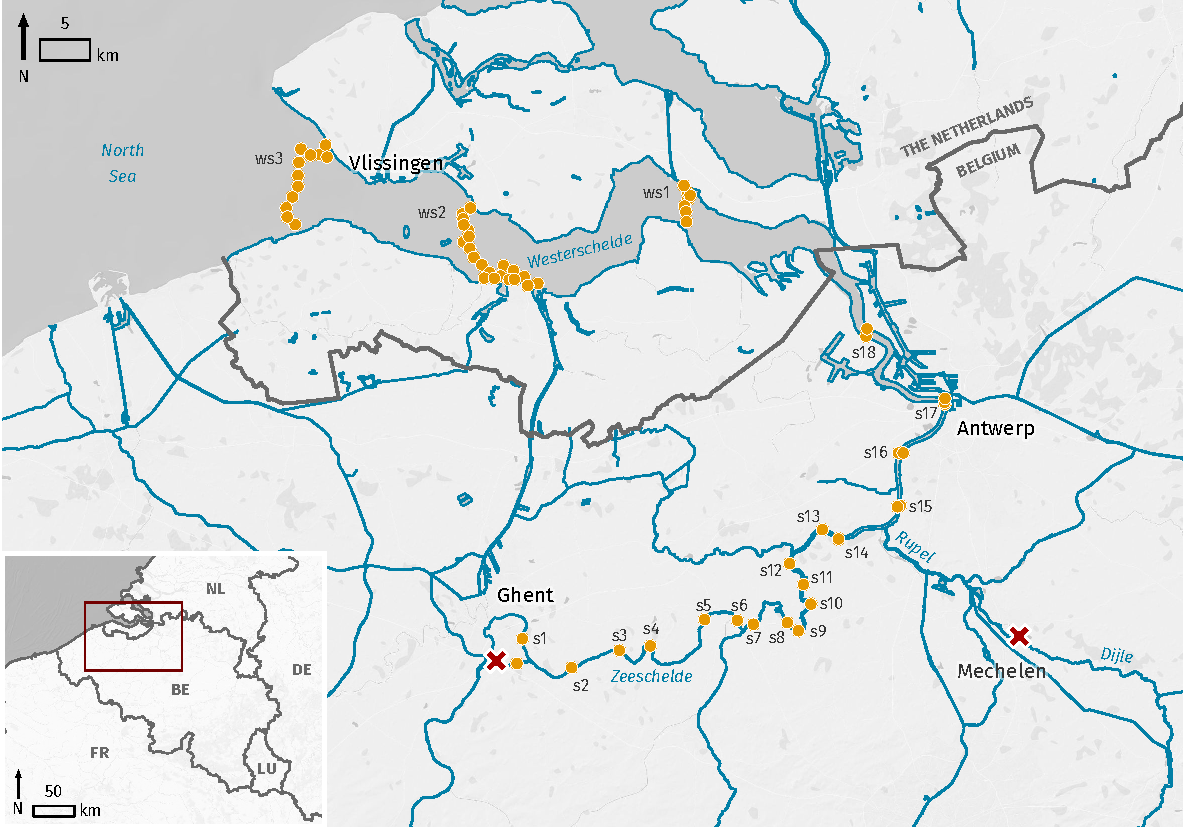
\includegraphics[scale=0.6]{receivernetwork.pdf}
  \caption{The Schelde Estuary comprises the Zeeschelde (Ghent-Antwerp) and Westerschelde (Antwerp-Vlissingen). Receivers are represented as orange circles. The gates are indicated as labels for different groups of receivers. The weir in Ghent and the weir in Mechelen where the eels and flounders were caught and released are depicted as red crosses. }
  \label{fig:network}
\end{figure}

The Schelde Estuary is a well-mixed estuary of 160 km long without transversal man-made migration barriers and characterized by strong currents, high turbidity and a large tidal amplitude up to 6 m \citep{Cornet2016}. The estuary can be divided in two regions (upstream to downstream): the Zeeschelde, which spans 105 km from Ghent to Antwerp (Belgium), and the Westerschelde, which covers the 55 km from Antwerp to the mouth of the estuary at Vlissingen (The Netherlands). The width of the Zeeschelde varies between 50 to 1350 m while the width of the Westerschelde varies between 2000 and 8000 m (Fig. \ref{fig:network}). 

\subsection{Tagging procedure}

At the tidal weir in Merelbeke (Ghent), 100 eels were caught and subsequently internally tagged with V13 (VEMCO Ltd., Canada) coded acoustic transmitters \citep{Verhelst2018}. After capture, surgery and recovery \citep{Thorstad2013b}, fish were released at the nearest receiver. Of the 100 tagged eels, 58 migrated and from these 58 eels, 38 started their migration from Ghent and reached Antwerp. The migration period of these 38 eels was determined \citep{Verhelst2018} and used for further analysis. We additionally tagged four flounders at the weir in Mechelen of the Dijle river, a tributary of the Scheldt estuary via the Rupel, with external V7 tags to assess whether the detection probability of the network is tag type and/or species specific. Since the factors species and tag type were confounded, it was not possible to determine which factor was responsible for observed differences. A more detailed description of the tagging procedure is provided in \ref{Taggingprocedure}.  

\subsection{Acoustic network}

Within the framework of the Belgian LifeWatch observatory, a permanent longitudinal network of receivers (VR2W, VEMCO Ltd, Canada) has been deployed since the spring of 2014 in the Schelde Estuary \citep{Reubens2019TheNetwork}. Currently, the network consists of 64 receivers which were combined into 21 gates (Table \ref{gate list}). In the Westerschelde, 39 receivers are moored on marine navigational buoys in three gates, which are in fact three bands of receivers stretching from shore to shore (from east to west: ws1: six receivers, average interdistance: 800 m; ws2: 21 receivers, average interdistance: 909 m and ws3: 12 receivers, average interdistance: 1132 m) (Fig. \ref{fig:network}). In the Zeeschelde, 25 receivers are deployed from the river bank. These 25 receivers are combined in 18 gates, which are on average 4969 m apart. At four locations (s15, s16, s17 and s18), a receiver on each side of the estuary was deployed to cover the whole width. The exact detection range for the different receivers in both the Westerschelde and Zeeschelde was unknown, but ranges between 300 m and 1000 m. Results from the network in the North Sea suggest that it is strongly dependent on current strength and wave action and will therefore be characterized by a strong spatial and temporal variability \citep{Reubens2018}.

\subsection{Data processing and analysis}

\subsubsection{Detection probability}

The detection probability was estimated using the conditional nature of fish movement throughout the system \citep{Brownscombe2019ConductingManagers}. Since there are no other pathways to the North Sea, tagged fish have to pass the different gates in a well-defined order and detection probability can be defined as the probability of detecting a tag moving past a specific gate \citep{Melnychuk2012,Perry2012UsingData}. The estimated detection probability was adjusted for any malfunctioning receivers or receivers that were installed later. Since the width of the Zeeschelde at the different gates is on average 236 meter and the detection range lies between 300 and 1000 meter, it is expected that the receivers will provide good coverage from shore to shore. However, in the Westerschelde, where the distance between the receivers of a single gate is on average 960 meter, it is expected that the coverage will be considerably less. We assumed that tagged fish only reach the North Sea when they are detected a the last gate or at the network of the North Sea. The network in the North Sea, which consists of 27 receivers scattered over a surface of 3,454 km$^2$, provided detections for six out of the 38 eels. Three of them were detected at the last gate too, but the other three were able to pass the last and second last gate undetected. The detection probabilities in the Zeeschelde and Westerschelde were 97.0 \% and 62.5 \% respectively while the overall detection probability was 95.5 \%. An estimate of the detection probability under the assumption that tagged fish reach the North Sea either way, even when they are not detected at any of the last three gates, is given in \ref{tab:det.prob.cases}.

\subsubsection{Residencies-at-receivers and residencies-between-receivers}

The main difference between the at-receivers and between-receivers approach, is the way in which detections are grouped in detection groups. For the at-receivers approach, all successive detections at one gate with a time lapse between them smaller than the absence threshold, are grouped. The summed time lapses of all these detection groups for one gate yield the residency at that specific gate of receivers (i.e. residency-at-receivers).  
For the between-receivers approach, the time lapse between the detections is of no interest to group the detections. The main difference between the detection groups is whether the detections occurred at one gate or at two different gates (Fig. \ref{fig:detectionInterval}). 
If two successive detections occur at different gates, these detections are grouped in pairs. It does not matter whether these gates are neighboring (type 1A) or not (type 1B). The time lapse between these detections indicates the duration that the tagged animal spent between the two gates. 
If successive detections occur at the same gate, those are grouped as well. Such a detection group resembles those estimated for the at-receivers approach, but with an infinite absence threshold. The time lapse between these detections indicates the duration that the tagged animal spent between the active gates (given that their detection probability is acceptable) neighboring the gate of interest as we do not know at which side of the latter the fish is located. The summed time lapses of all these detection groups for the area between two gates yield the residency between those specific gates of receivers (i.e. residency-between-receivers). 

\begin{figure}[h!]
  \centering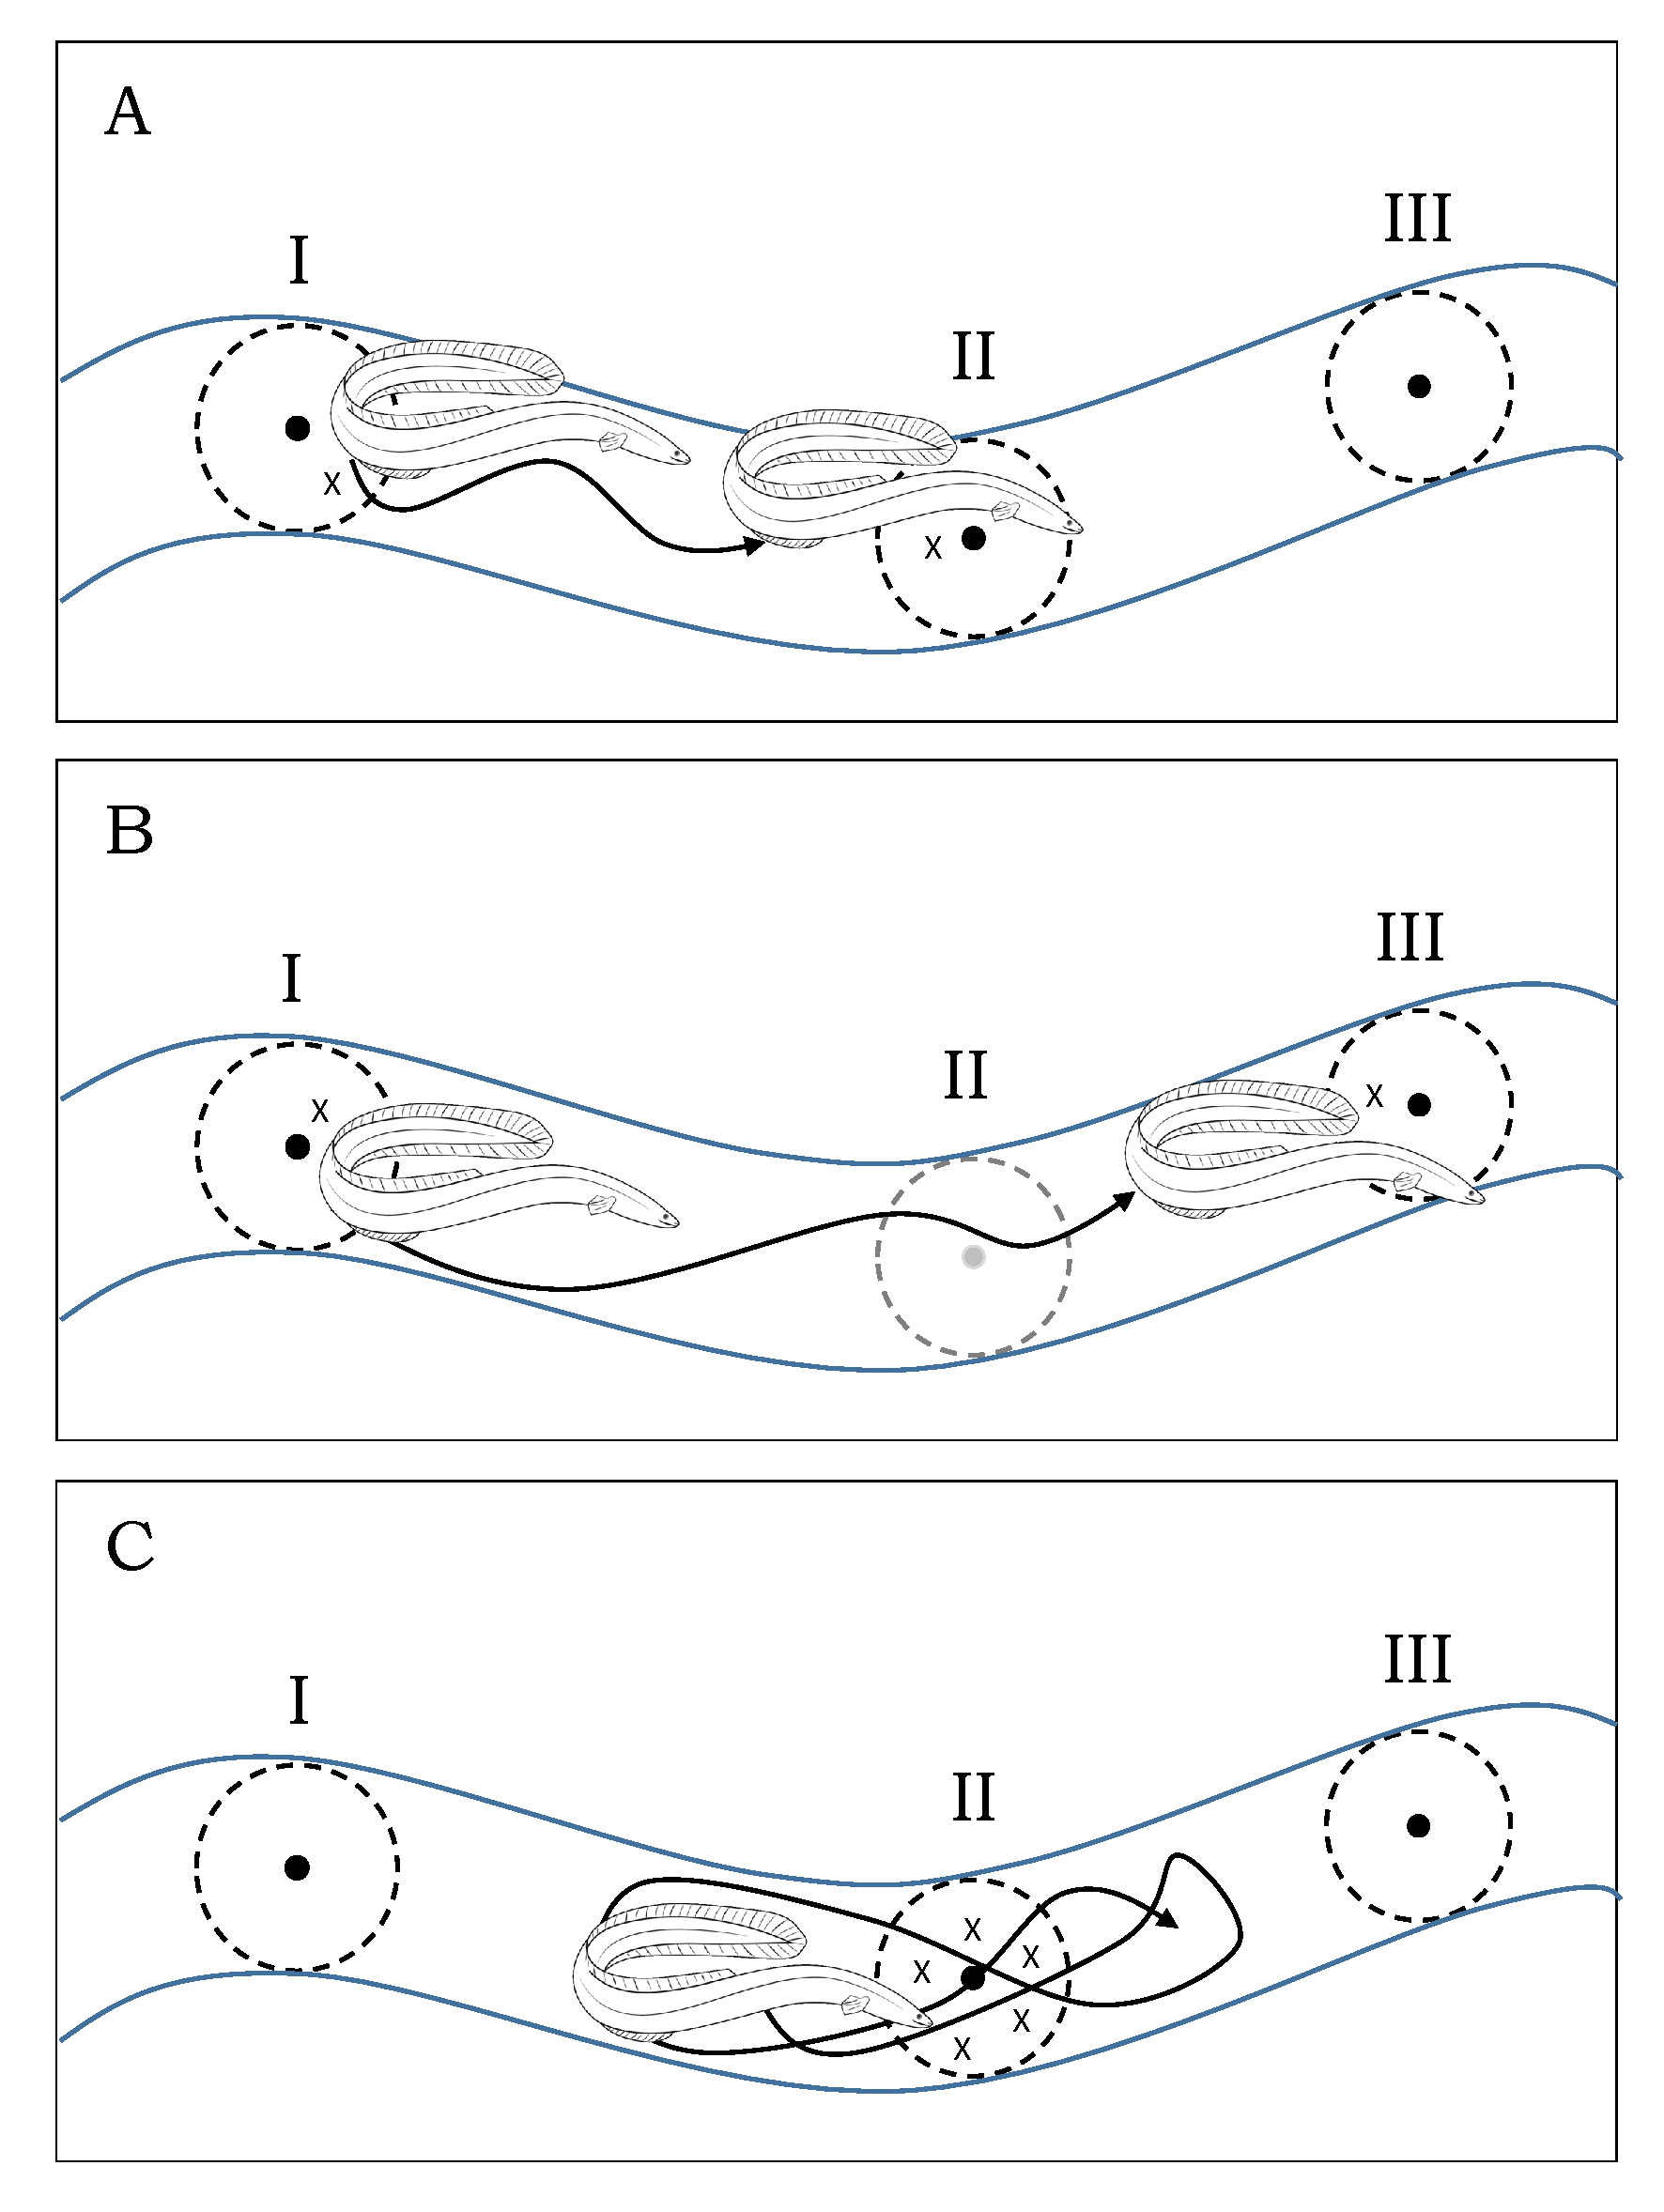
\includegraphics[scale=0.25]{figure_detection_intervals.pdf}
  \caption{Distinction between the different types of detection groups. Three different gates \RNum{1}, \RNum{2} and \RNum{3} (black points) with their corresponding detection ranges (dotted circles) are visualized in a river stretch. A cross depicts a detection at the concerning gate. In A, detection group type 1A is depicted. It consists of a pair of subsequent detections at two different neighboring gates. In B, detection group type 1B is depicted. It consists of a pair of subsequent detections at two different non-neighboring gates. In C, detection group type 2 is depicted. It consists of a group of at least two subsequent detections at one gate.}
  \label{fig:detectionInterval}
\end{figure}

Since some detection groups overlap in space and may contain multiple gates, tagged animals cannot always be positioned with certainty between two neighboring gates at a specific moment in time. Instead they may be positioned with certainty between non-neighboring gates which are located further apart. Therefore a specific residency-between-receivers will often not be estimated exactly, but will fall within an interval of possible values. The range of this interval is referred to as the epistemic uncertainty. A more practical example is given in \ref{Dataprocessing}. As the main aim of this study was to assess epistemic uncertainty, the statistical uncertainty arising from detection probabilities lower than 100 \% in combination with stochastic animal movement was not integrated in the uncertainty estimates described in this study. 

The residencies-between-receivers were divided by the distance between the gates for two reasons. First, as a means of normalization. Second, to allow for a comparison with the residencies-at-receivers, since the residencies-at-receivers are actually the estimated durations within a short-term activity area. The actual surface of the short-term activity area cannot be quantified as it is dependent on both the detection range and the absence threshold, but it may be considered constant if the detection range and absence threshold are assumed to be linearly related to the short-term activity area. 

To determine the trade-off between gate network resolution, or the percentage of sections between gates included, and epistemic uncertainty, all different combinations of sections bordered by gates were assessed. For every gate network resolution, different combinations could be constructed. For every fish and every gate network resolution the combination with the lowest average epistemic uncertainty was retained. A more elaborate example of the methodology is provided in \ref{Dataprocessing}. A linear mixed effects model with log-transformed epistemic uncertainty as response, gate network resolution as fixed effect and eel as random effect was constructed. A similar approach of evaluating epistemic uncertainty against gate network resolution was used to evaluate the effect of omitting specific gates from the network entirely (\ref{Fig}). 

\subsubsection{Comparison of the at-receivers and between-receivers approach}

Although the at-receivers approach and between-receivers approach are conceptually different, their relative results should be comparable. Both approaches are used to estimate the duration that tagged fish spend in specific areas. To this end, for each residency at a specific gate the corresponding residency-between-receivers was determined as the duration per unit of distance between the two neighboring gates of the gate at stake. At first glance there might seem to be a mismatch in the units used for the residencies-between-receivers (hours per 100 meter) and residencies-at-receivers (hours). However, as mentioned earlier, a residency-at-receivers is actually the duration that a tagged fish spent in an unknown but presumedly constant short-term area of activity. Rather than selecting an arbitrary value for this area, we have chosen to underline this limitation by not doing so. The detection range could be a good proxy for the short-term area of activity, but because of its earlier mentioned variable nature in the study area it was not included in this study. 

Because of the spatial overlap of the detection groups, the actual value of a residency-between-receivers cannot always be determined exactly. Instead an interval of possible values, i.e. epistemic uncertainty, is determined. Because the nature of the probability distribution of the intervals was considered unknown, Monte Carlo permutations were used to compare the residency-between-receivers intervals with the corresponding residencies-at-receivers, which could be estimated exactly. 10$^{6}$ repeats for each absence threshold, ranging from 0 to 100 hours in steps of one hour, were used to randomly select values from each residency-between-receivers interval. Pearson's correlation coefficients (\textit{r}) of each simulation were determined. R statistical software (version 3.5.0, R Developer Core Team, R Foundation for Statistical Computing, Vienna, Austria, https://www.R-project.org) was used.  

\section{Results}

\subsection{Residencies-between-receivers}

The trade-off between epistemic uncertainty and gate network resolution of different gate combinations of different tagged eels is depicted in Fig. ~\ref{fig:Pareto}. The output of the linear mixed effects model confirms a significant positive effect of reducing the gate network resolution on the epistemic uncertainty (Table \ref{tab:Mixed_Model}). The logarithmic relationship between uncertainty and resolution illustrates that a small reduction in resolution can have a large positive effect on the uncertainty.

\begin{figure}[h!]
  \centering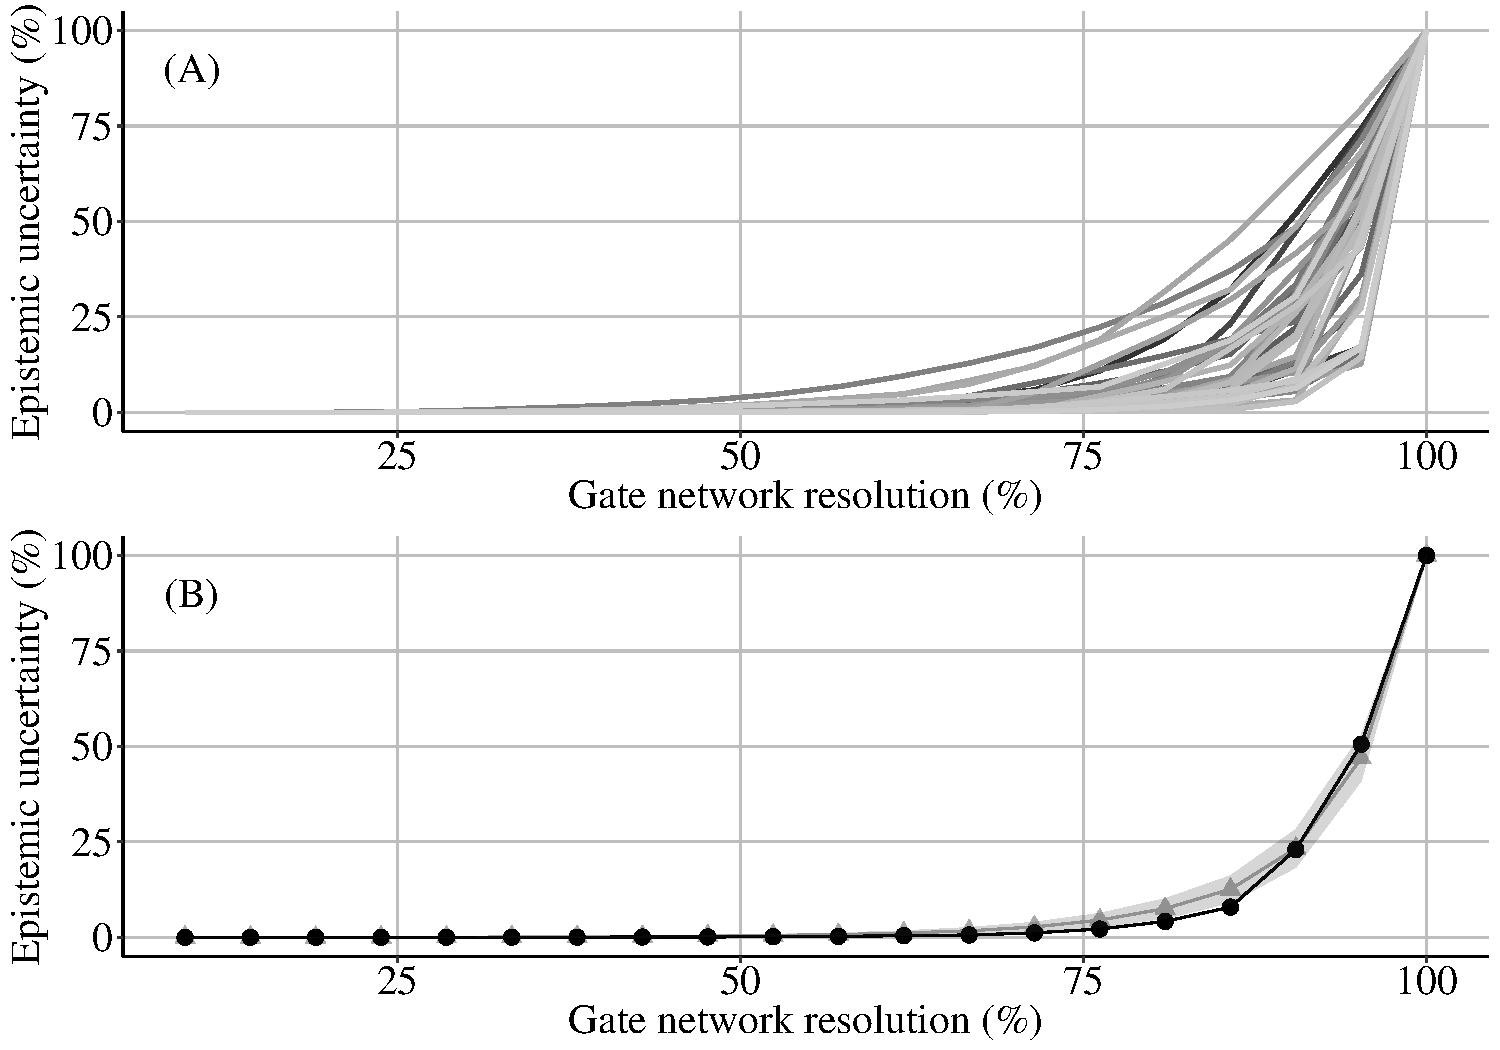
\includegraphics[scale=0.4]{Pareto_combo_final_grey_jb.pdf}
  \caption{Trade-off between normalized epistemic uncertainty (vertical axis) and gate network resolution (horizontal axis). Epistemic uncertainty was normalized for visualization purposes. In (A) this trade-off is given for all tagged eel separately, while in (B) the average (gray; triangle) and median (black; circle) trade-offs are visualized. The 95\% confidence interval of the average trade-off is visualized as a gray envelope.}
  \label{fig:Pareto}
\end{figure}

\begin{table}[h!]
\centering
\scriptsize
\caption{Output of the fixed effects of the linear mixed effects model with log-transformed epistemic uncertainty as response, gate network resolution as fixed effect and eel as random effect. The values, standard errors (SE), degrees of freedom (DF), t-values and p-values are given.}
\begin{tabular}{|l|l|l|l|l|l|} 
\hline
Fixed effect~         & Value    & SE      & DF   & t-value & p-value            \\ 
\hline
intercept             & -10.12207 & 0.1459427 & 636 & -69.35648 &       0            \\ 
\hline
Resolution            & 0.1225233 & 0.001078145 & 636 & 113.64265 &      0  \\
\hline
\end{tabular}
\label{tab:Mixed_Model}
\end{table}

On average, combining two sections, which coincides in our setting with a reduction in gate network resolution of 5 \%,  leads to an average decrease in epistemic uncertainty of 47 \%. Reducing the gate network resolution by 10, 15 and 20 \% leads to an average reduction in epistemic uncertainty of 72, 84 and 90 \% respectively. The optimal combination of sections for a specific gate network resolution differed between tagged eels. Therefore, one tagged eel was randomly selected to illustrate the principle of combining sections in an optimal way  (Fig.~\ref{fig:Resistance_model} and Fig. \ref{fig:Flow_chart}). In appendix, more examples for different eels are given (Fig. \ref{fig:Resistance_model2} and Fig. \ref{fig:Resistance_model3}) and a suggestion is provided on how to obtain an overview of the entire population (Fig. \ref{fig:overall_uncertainty}). In Fig. \ref{fig:Resistance_model_flounder}, the principle of combining sections in an optimal way is given for one out of four randomly selected flounders.

\begin{figure}[h!]
  \centering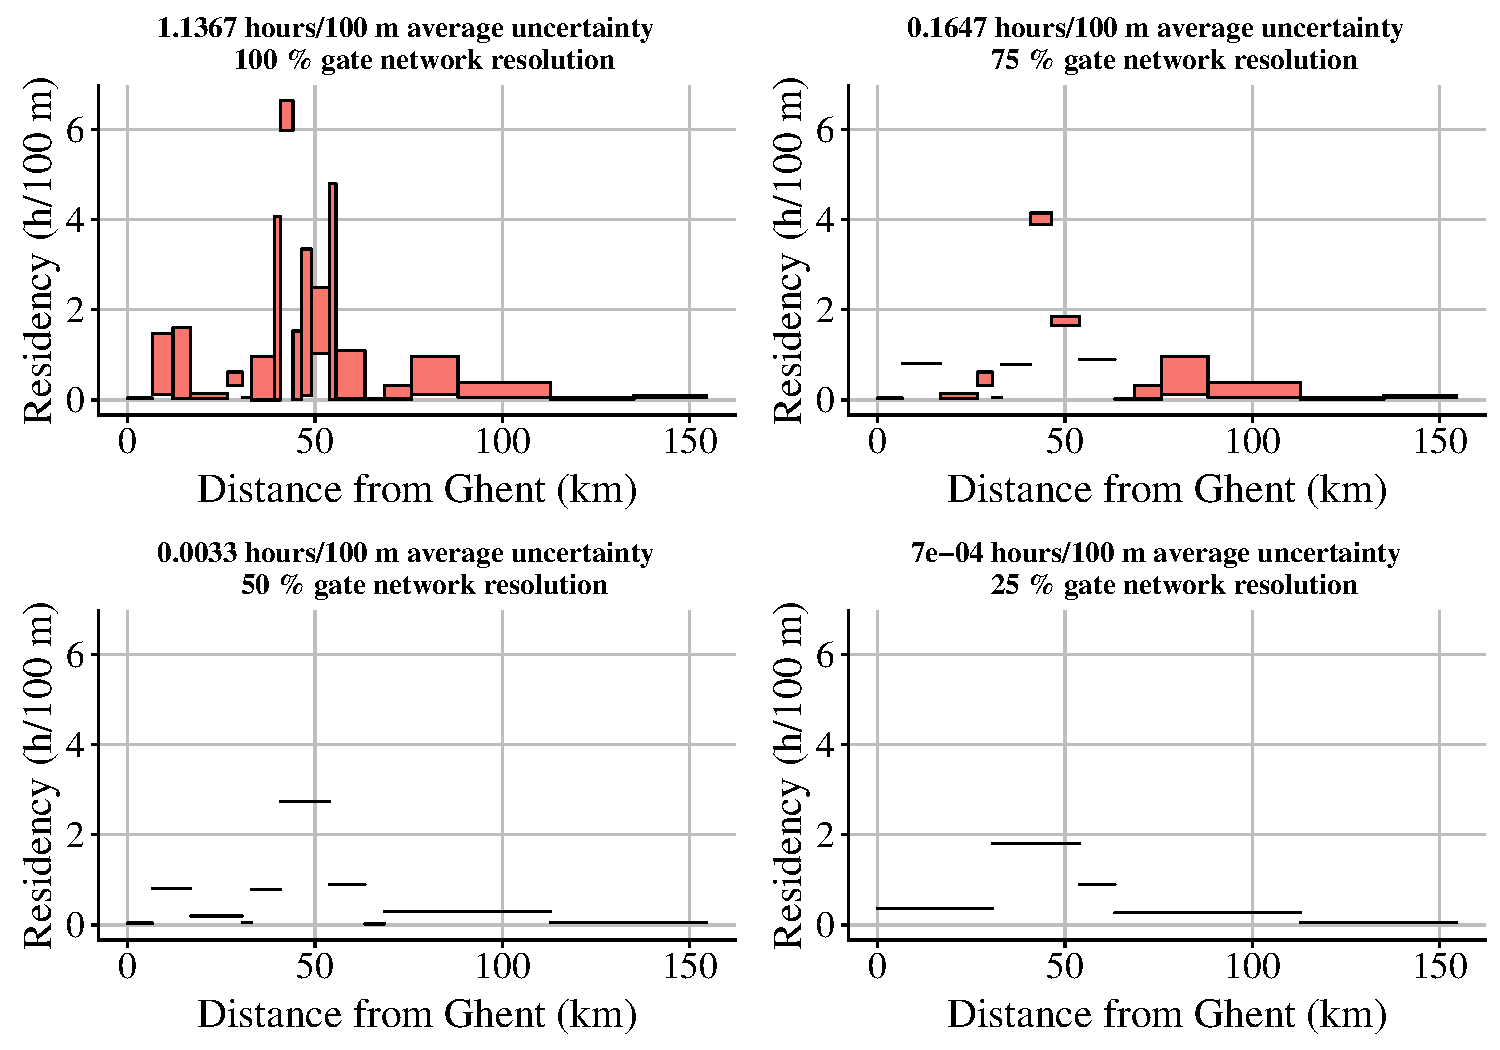
\includegraphics[scale=0.45]{Resistance_model2_jb_eel.pdf}
  \caption{Residency-between-receivers (hours/100m) in function of distance from Ghent (km). Combinations of sections bordered by gates for eel "A69-1601-52622" with different levels of gate network resolution and different levels of average epistemic uncertainty are depicted. The range between the minimum and maximum value of the residencies-between-receivers, i.e. the epistemic uncertainty, is represented by the red boxes.}
  \label{fig:Resistance_model}
\end{figure}

\begin{figure}[h!]
  \centering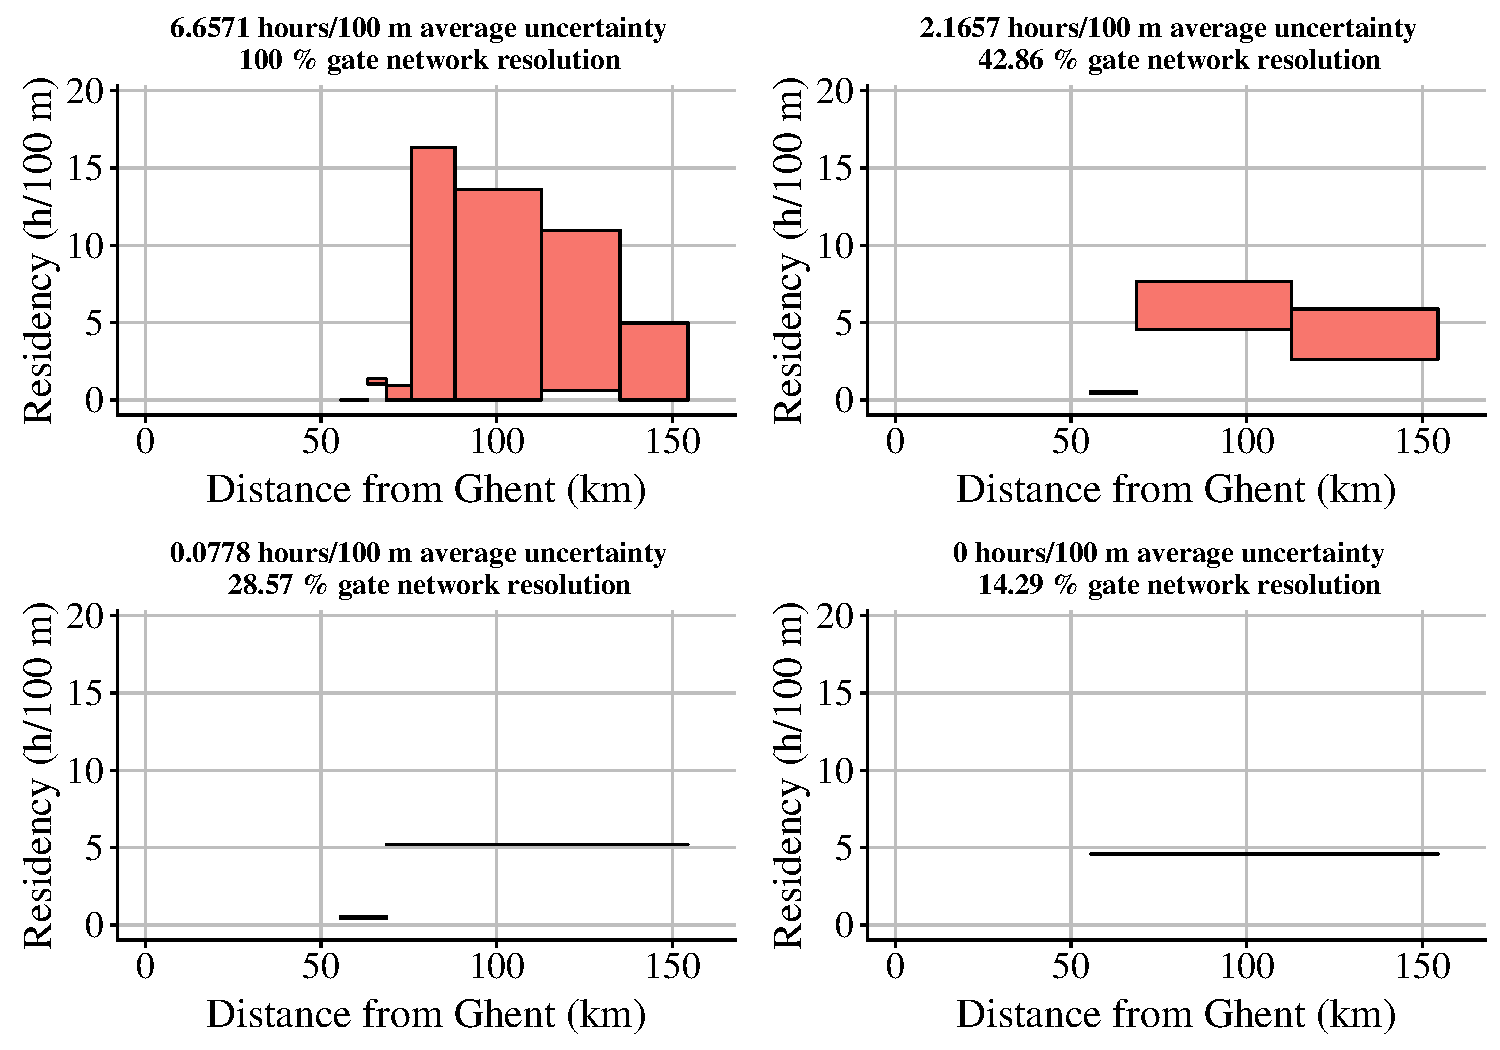
\includegraphics[scale=0.45]{flounder_res_model_jb.pdf}
  \caption{Residency-between-receivers (hours/100m) in function of distance from Ghent (km). Combinations of sections bordered by gates for flounder "A69-1601-34454" with different levels of gate network resolution and different levels of average epistemic uncertainty are depicted. The range between the minimum and maximum value of the residencies-between-receivers, i.e. the epistemic uncertainty, is represented by the red boxes.}
  \label{fig:Resistance_model_flounder}
\end{figure}

The linear mixed effects model revealed a significant negative effect on the epistemic uncertainty of omitting a gate from the analysis (\textit{p}<0.05) (Table \ref{lmer model stations removed} and Fig. \ref{fig:Pareto_stations_removed}). Post-hoc tests with Bonferroni correction revealed that the removal of Gates ws2, ws1, s4 and s12 lead to a significantly higher epistemic uncertainty than the removal of Gates s10 and s11. 

\subsection{Comparison of the at-receivers and between-receivers approach}

The linear correlation between residencies-at-receivers and corresponding residencies-between-receivers was weak with Pearson's correlation coefficient ranging from 0.33 to 0.45. The absence threshold did not have a meaningful effect on this, although the correlation seemed to improve slightly with increasing absence threshold. This is probably because the residencies-at-receivers became more similar to the type 2 detection groups of the between-receivers approach (Figure \ref{fig:correlation}). After 70 hours this trend stabilized because eel did not spend more than 70 hours between two gates. 

\begin{figure}[h!]
  \centering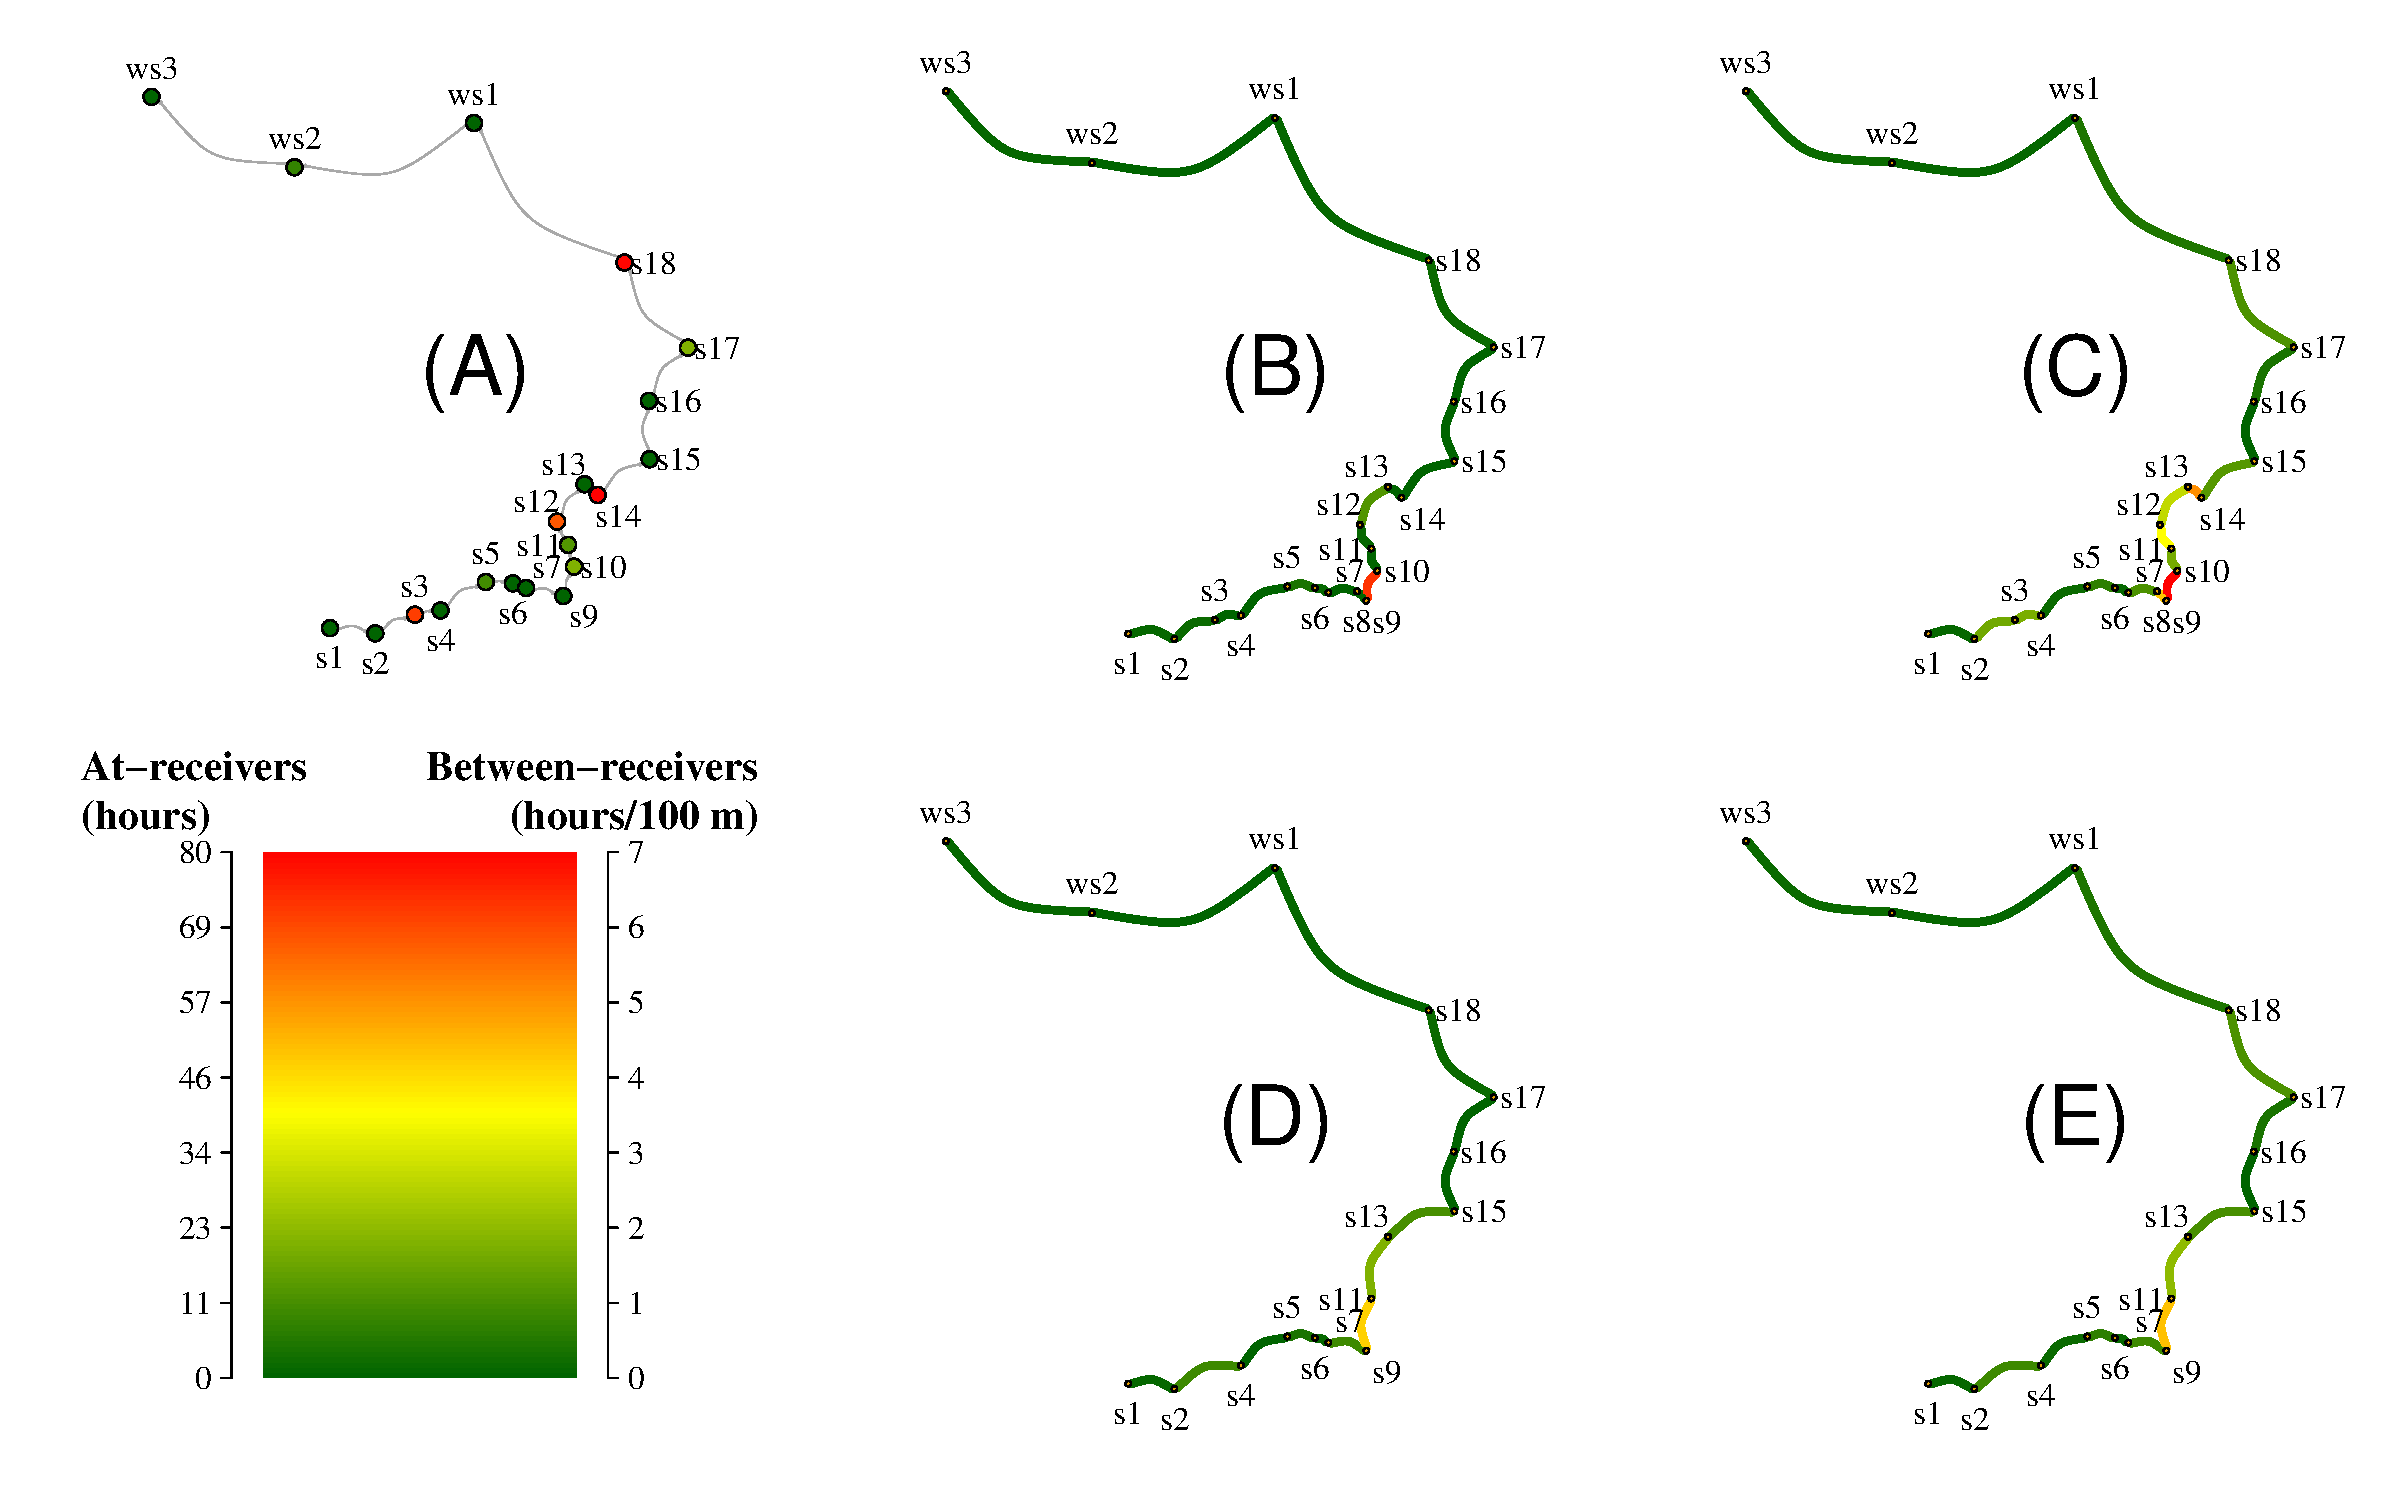
\includegraphics[scale=0.35]{Map_Network_Analysis.pdf}
  \caption{These maps visualize the residencies in the network of the Schelde Estuary of one tagged eel "A69-1601-52622". Gates are represented as nodes and the sections between the gates are represented as lines. In (A) the estimated residencies-at-receivers (absence threshold of 70 hours) are depicted. In (B) and (C) the estimated minimum and maximum, respectively, of the residency-between-receivers intervals are visualized. This combination of sections bordered by gates has an average epistemic uncertainty of 1.1367 hours/100 meter and a gate network resolution of 100 \% (Fig. \ref{fig:Resistance_model}). Figures (D) and (E) also represent the minimum and maximum, respectively, of the residency-between-receivers intervals. This combination has an average epistemic uncertainty of  0.1647 hours/100 meter and a gate network resolution of 75 \% (Fig. \ref{fig:Resistance_model}).}
  \label{fig:Map_Network_Analysis}
\end{figure}

Maps of the estimated residencies-at-receivers (absence threshold of 70 hours) of tagged eel "A69-1601-52622" were constructed (Fig.~\ref{fig:Map_Network_Analysis} (A)) to visually compare with the outcomes of the section combinations of the concerning tagged eel using the between-receivers approach. In Fig.~\ref{fig:Map_Network_Analysis} (B) and Fig.~\ref{fig:Map_Network_Analysis} (C), respectively, the minimum and maximum values of the residency-between-receivers intervals of a combination with a gate network resolution of 100 \% are visualized. A large difference between the minimum and maximum value corresponds with a high epistemic uncertainty. The epistemic uncertainty reduces significantly (\textit{p}<0.05; Table \ref{tab:Mixed_Model}) when lowering the gate network resolution by 25 \% as can be seen in Fig.~\ref{fig:Map_Network_Analysis} (D) and Fig.~\ref{fig:Map_Network_Analysis} (E). 

\section{Discussion}
\label{Disc}

\subsection{Assessment of a passive acoustic telemetry network}
\label{subsec:Assessment of a passive acoustic telemetry network}

The success of this approach to determine the approximate position of tagged individuals at any time and to assess the epistemic uncertainty, strongly depends on the detection probability \citep{Heupel2006,Melnychuk2012,Reubens2018}. If tagged fish are able to pass certain gates without being detected, uncertainty may actually be higher than estimated, because gates are assumed to have a perfect detection probability. Gates with low detection probabilities should therefore be treated with care. Although Gate ws3 had a low detection probability (45.16 \%), it was still considered as a valuable gate since the long stretch of the Westerschelde has only a limited number of gates. 

Since maintaining networks is expensive  and network assessment methods are limited, a standardized approach to optimize the telemetry network is invaluable \citep{Steckenreuter2017,Kraus2018}. In this study it turned out that the simulated removal of any gate had a significant effect on the epistemic uncertainty. When omitting a gate from the network, the epistemic uncertainty increases (Figure \ref{fig:Pareto_stations_removed}). The stronger this increase, the more important the gate. The removal of Gates ws2, ws1 and s12 had a bigger impact on the epistemic uncertainty than the removal of Gates s10 and s11. This is probably because of the low detection probabilities of the surrounding gates of Gates ws2, ws1 and s12 which contribute to more spatially overlapping detection groups, invoking higher levels of epistemic uncertainty. When selecting a gate for removal one should also take into account other aspects besides epistemic uncertainty such as the detection probability itself and the coverage of potentially interesting river stretches. For example, removing Gates ws2 and ws1 might not be the preferred option in terms of epistemic uncertainty, but it could be in terms of detection probability and required number of receivers (see further). 

In case the detection probability is relatively low, epistemic uncertainty can be very high \citep{Melnychuk2012}. This was for example the case for flounder (Fig. \ref{fig:Resistance_model_flounder}) where average detection probability was only 39.17 \% (Table \ref{gate list}) and average epistemic uncertainty was $2.43\,\pm $2.73 (SD) while for eel this was 90.71 \% and $0.99\,\pm $0.70 (SD) respectively. Although the number of studied flounder individuals was limited, the low detection probability of flounder compared to eel, indicates that a species and/or tag-type specific assessment of the network is necessary to optimally process the data. To improve the detection probability more receivers could be positioned more closely to one another, higher power tags could be used, or the intervals between tag pulses could be reduced \citep{Clements2005}. For example, three out of the 38 tagged eels had a tag with a lower power output and two of them had the lowest and second lowest detection probability respectively (Table \ref{tag_list}).

\subsection{Residencies-between-receivers}
 
To this day, telemetry studies focusing on the epistemic uncertainty of position estimates in aquatic environments have been few \citep{Pedersen2013,Roy2017,Steckenreuter2017}. However, to locate migration barriers and home ranges, researchers need to be aware of the time animals spend on and between locations and to do so they require sound statistical methods, which are able to quantify the uncertainty tied up with imperfect data. The estimated residencies-between-receivers allow to assess the time that each fish spends within every combination of sections bordered by gates. The large range of a residency-between-receivers interval indicated a large uncertainty regarding the real time spent between gates. Combinations with a lower gate network resolution, had a significantly lower average uncertainty (Figure \ref{fig:Pareto}). Reducing the gate network resolution from 100 to  80 \% decreased the average epistemic uncertainty from 100 to 10 \%. The reason for this is twofold. First, the reduction in gate network resolution resulted in more gates being within the different sections. These gates did not serve as detection borders to allocate position estimates to a specific section, but validated the position estimates within different sections. Second, combining the sections was not done haphazardly. For each unit decrease of gate network resolution, the combination with the lowest uncertainty and lowest amount of overlapping detection groups was retained. 

When researchers decide to reduce epistemic uncertainty at the cost of the gate network resolution, results will be less conclusive, but more reliable. Therefore, combinations with high gate network resolutions may be faced with too high an epistemic uncertainty to make sound conclusions, compared to combinations with lower gate network resolutions (Figure \ref{fig:Map_Network_Analysis}). The optimal trade-off is context dependent and different criteria in addition to epistemic uncertainty and gate network resolution should be considered to arrive at the most suitable combination. For example, users could choose to penalize gate combinations with a high epistemic uncertainty in specific areas and/or during specific periods, they could choose to improve the gate network resolution locally to better fit the research objectives or they could integrate the distance between gates and the detection probability in the selection process of section combinations. 

\subsection{Comparison of the at-receivers and between-receivers approach}

In passive acoustic telemetry studies, networks rarely have a full coverage, tagged animals are not located continuously and researchers need to predict where the animals reside while not being detected \citep{Heupel2006,Hedger2008,Trancart2017}. Currently used data processing methods based on residencies-at-receivers are strongly dependent on biological assumptions; if tagged fish are repeatedly detected within a time span below the absence threshold, they are presumed to reside in the area of the concerned receiver \citep{Vokoun2003}. Since the aim of most telemetry studies is to describe yet unknown biological features \citep{Hussey2015} and given the unpredictable nature of wildlife, making biological assumptions might be ambiguous. To predict the position of tagged animals, the between-receivers approach depends more strongly on the characteristics of the network, rather than on the characteristics of the animals themselves. As mentioned in Section \ref{subsec:Assessment of a passive acoustic telemetry network}, detection probability is key to successfully implement this approach. Hence, for large open areas, such as seas, where a large number of receivers is required to serve as gate, this method is less suitable \citep{Hobday2011EstimatingArrays}. For example, in the Westerschelde, which is between 2000 and 8000 m wide, on average 13 receivers per gate yield a detection probability of only 63.78 \%. In contrast, in the Zeeschelde, which is between 50 and 1350 m wide, on average 1.28 receivers per gate yield a detection probability of 96.61 \%.  

The residencies-at-receivers obtained through absence thresholds turned out to be only poorly correlated (Pearson's \textit{r} ranging from 0.33 to 0.45) to the residencies-between-receivers (Fig. \ref{fig:correlation} and Fig. \ref{fig:Map_Network_Analysis}). In addition, the effect of the absence threshold itself turned out to be negligible. Therefore, the inability of the residencies-at-receivers to serve as a proxy for the time spent within a certain section, in combination with the lacking quantification of the epistemic uncertainty, underline the importance of the proposed approach based on gates. The preference for the between-receivers approach over the at-receivers approach in longitudinal aquatic systems may be intuitive, but the ability to quantify its added value can support researchers to decide on the design of their telemetry network. 

\subsection{Suggestions to integrate both epistemic and statistical uncertainty}

Since the main aim of this study was to quantify and reduce epistemic uncertainty, statistical uncertainty, which is the result of imperfect detectability, was not considered. However, in case detection probabilities are low, statistical uncertainty could be an important aspect to account for and methods that allow to integrate both types of uncertainty would be useful. Epistemic uncertainty is defined by a lack of knowledge and can therefore be reduced either by improving our understanding, e.g. more exact position estimates, or by balancing knowledge requirements, e.g. trade-off between spatial resolution and estimates of residency periods. Statistical uncertainty on the other hand is the sampling variability caused by the inherently irreducible stochasticity of detectability and animal movement \citep{Fox2011DistinguishingUncertainty}. Unlike epistemic uncertainty, for which only interval approximations can be determined, the statistical uncertainty can be described by probability distributions using traditional probabilistic methods \citep{Eldred2009EfficientElectronics}. As stochasticity is irreducible, the sampling variability or statistical uncertainty would not be reduced by the reduction of spatial resolution in the same way as the epistemic uncertainty. Instead, the rearrangement of gate sections would alter the gates serving as border to sections, affecting the detection probability of the network and as such statistical uncertainty

To quantify and potentially reduce the combined epistemic and statistical uncertainty, a second-probability analysis could be used \citep{Sundgren2013UncertaintyProbability}. In practice, an additional nested iteration would be added to the optimization scheme, with multiple sets of epistemic uncertainty values (outer-loop) yielding an equal amount of cumulative distribution functions (CDFs) based on the statistical uncertainty (inner-loop) \citep{Eldred2009EfficientElectronics}. The bounds of this collection of CDFs at different probability levels (e.g. 2.5 \% and 97.5 \% for a 95\% CI) can be calculated and used as a combined measure of uncertainty \citep{Eldred2009EfficientElectronics}. In addition, to account for the spatiotemporal variability of the detection probability and resulting statistical uncertainty, environmental measurements and detection-range tests could be used to develop models describing the relationship between environmental conditions, detection range and detection probability \citep{Mathies2014EnvironmentalArrays,Reubens2018}. In turn, the uncertainty of this detection range model would need to be accounted for in the uncertainty propagation. It should be noted that, because of the additional iterations, the suggested individual-based optimization scheme for mixed uncertainty estimates and spatial re-scaling will become computationally much more expensive \citep{Eldred2009EfficientElectronics}. Therefore, future studies should also focus on the assessment of different optimization schemes by comparing different stochastic expansion and interval optimization methods \citep{Han2014InherentActuators,Terejanu2010ApproximateSystems}. 

\section{Conclusion}

Although passive acoustic telemetry allows one to obtain extensive data sets of multiple individuals, different sources of temporal and spatial uncertainty are present. Being aware of the epistemic uncertainty of telemetry data and the practical limitations of telemetry networks is paramount to allow optimal use. This novel approach based on gates may introduce new challenges to interpret the data correctly, but has two major advantages. Epistemic uncertainty of acoustic telemetry networks can be quantified and reduced at the cost of some spatial information by using gates as validation centers rather than geographical boundaries to residency estimates. The currently used data processing methods are undoubtedly useful in large open areas, but in one-dimensional river stretches a less ambiguous approach should be used whenever possible. Although this study was limited to just one river stretch, the method can be easily extended to other networks of longitudinal aquatic systems. The method could be extrapolated to other telemetry techniques such as radio, PIT or NEDAP Trail telemetry. 

\section*{\ackname}

This work was supported by the Flemish branch of the LifeWatch ESFRI observatory. P. Verhelst acknowledges the support of the Flemish Agency for Innovation and
Entrepreneurship (VLAIO), now under the auspices of the National Science Fund FWO, during a large part of this study. R. Baeyens, N. De Maerteleire, S. Franquet, E. Gelaude, T. Lanssens, S. Pieters, K. Robberechts, T. Saerens, R. van der Speld, S. Vermeersch and Y. Verzelen assisted with the data collection. B. Lonneville aided in the creation of the map. This work makes use of data and infrastructure provided by VLIZ and INBO and funded by Research Foundation - Flanders (FWO) as part of the Belgian contribution to LifeWatch. We would also like to thank the Royal Belgian Institute of Natural Sciences, Operational Directorate Natural Environment (RHIB Tuimelaar) for infrastructure provision and Rijkswaterstaat (The Netherlands) for their cooperation and the permission to use their marine buoys.

\section*{\autcont}

S.B. conceived the ideas and designed methodology, analyzed the data and led the writing of the manuscript; P.V., J.R. and S.B. collected the data; All authors contributed critically to the drafts and gave final approval for publication.

\section*{\datacc}

The R code, subset of data and documentation are available on Mendeley Data: \url{http://dx.doi.org/10.17632/8b4m7b3jnc.1}

\newpage

\bibliographystyle{elsarticle-harv-noURL}
\bibliography{references}

\newpage
\FloatBarrier
\appendix

\section{Tagging procedure}
\label{Taggingprocedure}

\setcounter{table}{0} \renewcommand{\thetable}{A.\arabic{table}}
\setcounter{figure}{0} \renewcommand{\thefigure}{A.\arabic{figure}}

The following description is adapted from \citet{Verhelst2018}. 100 Eels were caught and tagged at the tidal weir in Merelbeke in the Zeeschelde during late summer and autumn (September–November) of three consecutive years (2015 till 2017) using double fyke nets. After periods of heavy rain, water flows over the sluices allowing eels to swim over the sluices. Placing the fyke nets behind the sluices and during periods of heavy rain, allowed to coordinate capture events and improve the chance of capturing eel. Several morphometric features were measured in order to determine the eel maturation stage \citep{Durif2005}: Total length (TL, to the nearest mm), body weight (W, to the nearest g), the vertical and horizontal eye diameter (EDv and EDh respectively, to the nearest 0.01 mm) and the length of the pectoral fin (FL, to the nearest 0.01 mm) (Table \ref{dimensionsTaggedEels}). Only females were tagged, since males are smaller than the minimum size handled in this study (< 450 mm \citep{Durif2005}). Eels of three different maturation stages were tagged: premigrant (F3, n = 51) and the two migrant stages F4 and F5 (n = 21 and n = 28, respectively). The eels were tagged with V13 coded acoustic transmitters (13 x 36 mm, weight in air 11 g, frequency 69 kHz, ping frequency: 60–100 s; estimated battery life: 1021-1219 days (battery life time depended on specific transmitter settings), (Table \ref{settingsTaggedEels})) from VEMCO Ltd (Canada). After anesthetizing them with 0.3 ml/L clove oil, tags were implanted with permanent monofilament \citep{Thorstad2013b}. Eels recovered in a quarantine reservoir for approximately one hour and were subsequently released at the nearest receiver. 

Four flounders were tagged with external V7 tags and released at the weir in Mechelen of the Dijle river, a tributary of the Scheldt estuary via the Rupel. A needle with nylon tread was used to attach the tag to the skin, just above the anal fin. The tag was attached on the dorsal side of the fish. Two rubber plates were attached on both sides of the fish to prevent rupture of the skin. On the dorsal side the rubber plate was attached between the skin and the tag. The tags were set to have a low power output and a ping frequency of 40 to 80 seconds.

\begin{table}[]
\centering
\scriptsize
\caption{Number of all tagged female eels per stage with the different morphometrics: total length (TL), body weight (BW), horizontal and vertical eye diameters (EDh and EDv, respectively) and pectoral fin length (FL). Mean, standard deviation and range (between brackets) are indicated (Adopted from \citet{Verhelst2018}).}
\label{dimensionsTaggedEels}
\begin{tabular}{|l|l|l|l|l|l|l|}
\hline
Stage & Number & TL (mm)                                                         & BW (g)                                                             & EDh (mm)                                                               & EDv (mm)                                                              & FL (mm)                                                                 \\ \hline
F3  & 51     & \begin{tabular}[c]{@{}l@{}}$702 \pm $57 \\ (568 - 835)\end{tabular} & \begin{tabular}[c]{@{}l@{}}$674 \pm $165 \\ (324 - 1106)\end{tabular}  & \begin{tabular}[c]{@{}l@{}}$8.08 \pm $0.57 \\ (6.77 - 9.08)\end{tabular}   & \begin{tabular}[c]{@{}l@{}}$7.55 \pm $0.60 \\ (6.20 - 9.70)\end{tabular}  & \begin{tabular}[c]{@{}l@{}}$32.92 \pm $3.29 \\ (26.76 - 40.32)\end{tabular} \\ \hline
F4   & 21     & \begin{tabular}[c]{@{}l@{}}$810 \pm $57 \\ (707 - 932)\end{tabular} & \begin{tabular}[c]{@{}l@{}}$1162 \pm $217 \\ (771 - 1830)\end{tabular} & \begin{tabular}[c]{@{}l@{}}$10.41 \pm $0.92 \\ (9.13 - 12.49)\end{tabular} & \begin{tabular}[c]{@{}l@{}}$9.66 \pm $0.78 \\ (8.60 - 11.86)\end{tabular} & \begin{tabular}[c]{@{}l@{}}$40.86 \pm $4.32 \\ (30.84 - 48.18)\end{tabular} \\ \hline
F5    & 28     & \begin{tabular}[c]{@{}l@{}}$662 \pm $56 \\ (575 - 775)\end{tabular} & \begin{tabular}[c]{@{}l@{}}$585 \pm $144 \\ (417 - 912)\end{tabular}   & \begin{tabular}[c]{@{}l@{}}$9.33 \pm $0.80 \\ (8.14 - 11.18)\end{tabular}  & \begin{tabular}[c]{@{}l@{}}$8.80 \pm $0.79 \\ (7.62 - 10.39)\end{tabular} & \begin{tabular}[c]{@{}l@{}}$34.41 \pm $3.68 \\ (28.97 - 45.37)\end{tabular} \\ \hline
\end{tabular}
\end{table}

\begin{table}[]
\centering
\scriptsize
\caption{The number and settings of the transmitters of all tagged eels per step: power output (PO; L = low power output, H = high power output), ping frequency (s) and the time duration (days) per step as well as the total battery life time (days). (Adopted from \citet{Verhelst2018})}
\label{settingsTaggedEels}
\begin{tabular}{|l|l|l|l|l|l|l|l|}
\hline
\multirow{2}{*}{\begin{tabular}[c]{@{}l@{}}Number \\ of \\ transmitters\end{tabular}} & \multicolumn{3}{l|}{Step 1}                                                                                                        & \multicolumn{3}{l|}{Step 2}                                                                                                        & \multirow{2}{*}{\begin{tabular}[c]{@{}l@{}}Battery \\ life \\ (days)\end{tabular}} \\ \cline{2-7}
                                                                                      & PO & \begin{tabular}[c]{@{}l@{}}Ping \\ frequency \\ (s)\end{tabular} & \begin{tabular}[c]{@{}l@{}}Duration \\ (days)\end{tabular} & PO & \begin{tabular}[c]{@{}l@{}}Ping \\ frequency \\ (s)\end{tabular} & \begin{tabular}[c]{@{}l@{}}Duration \\ (days)\end{tabular} &                                                                                    \\ \hline
20                                                                                    & L  & 60 - 100                                                         & 1216                                                       & NA & NA                                                               & NA                                                         & 1216                                                                               \\ \hline
40                                                                                    & H  & 60 - 100                                                         & 120                                                        & L  & 60 - 100                                                         & 901                                                        & 1021                                                                               \\ \hline
40                                                                                    & H  & 60 - 100                                                         & 120                                                        & L  & 60 - 100                                                         & 902                                                        & 1022                                                                               \\ \hline
\end{tabular}
\end{table}

\begin{table}[]
\centering
\scriptsize
\caption{Total length (TL) and body weight (BW) of the tagged flounders}
\label{dimensionsTaggedFlounder}
\begin{tabular}{|l|l|l|}
\hline
Transmitter    & TL (mm) & BW (g) \\ \hline
A69-1601-34454 & 261     & 282    \\ \hline
A69-1601-34455 & 298     & 272    \\ \hline
A69-1601-34456 & 315     & 376    \\ \hline
A69-1601-34460 & 339     & 496    \\ \hline
\end{tabular}
\end{table}

\begin{figure}[h!]
  \centering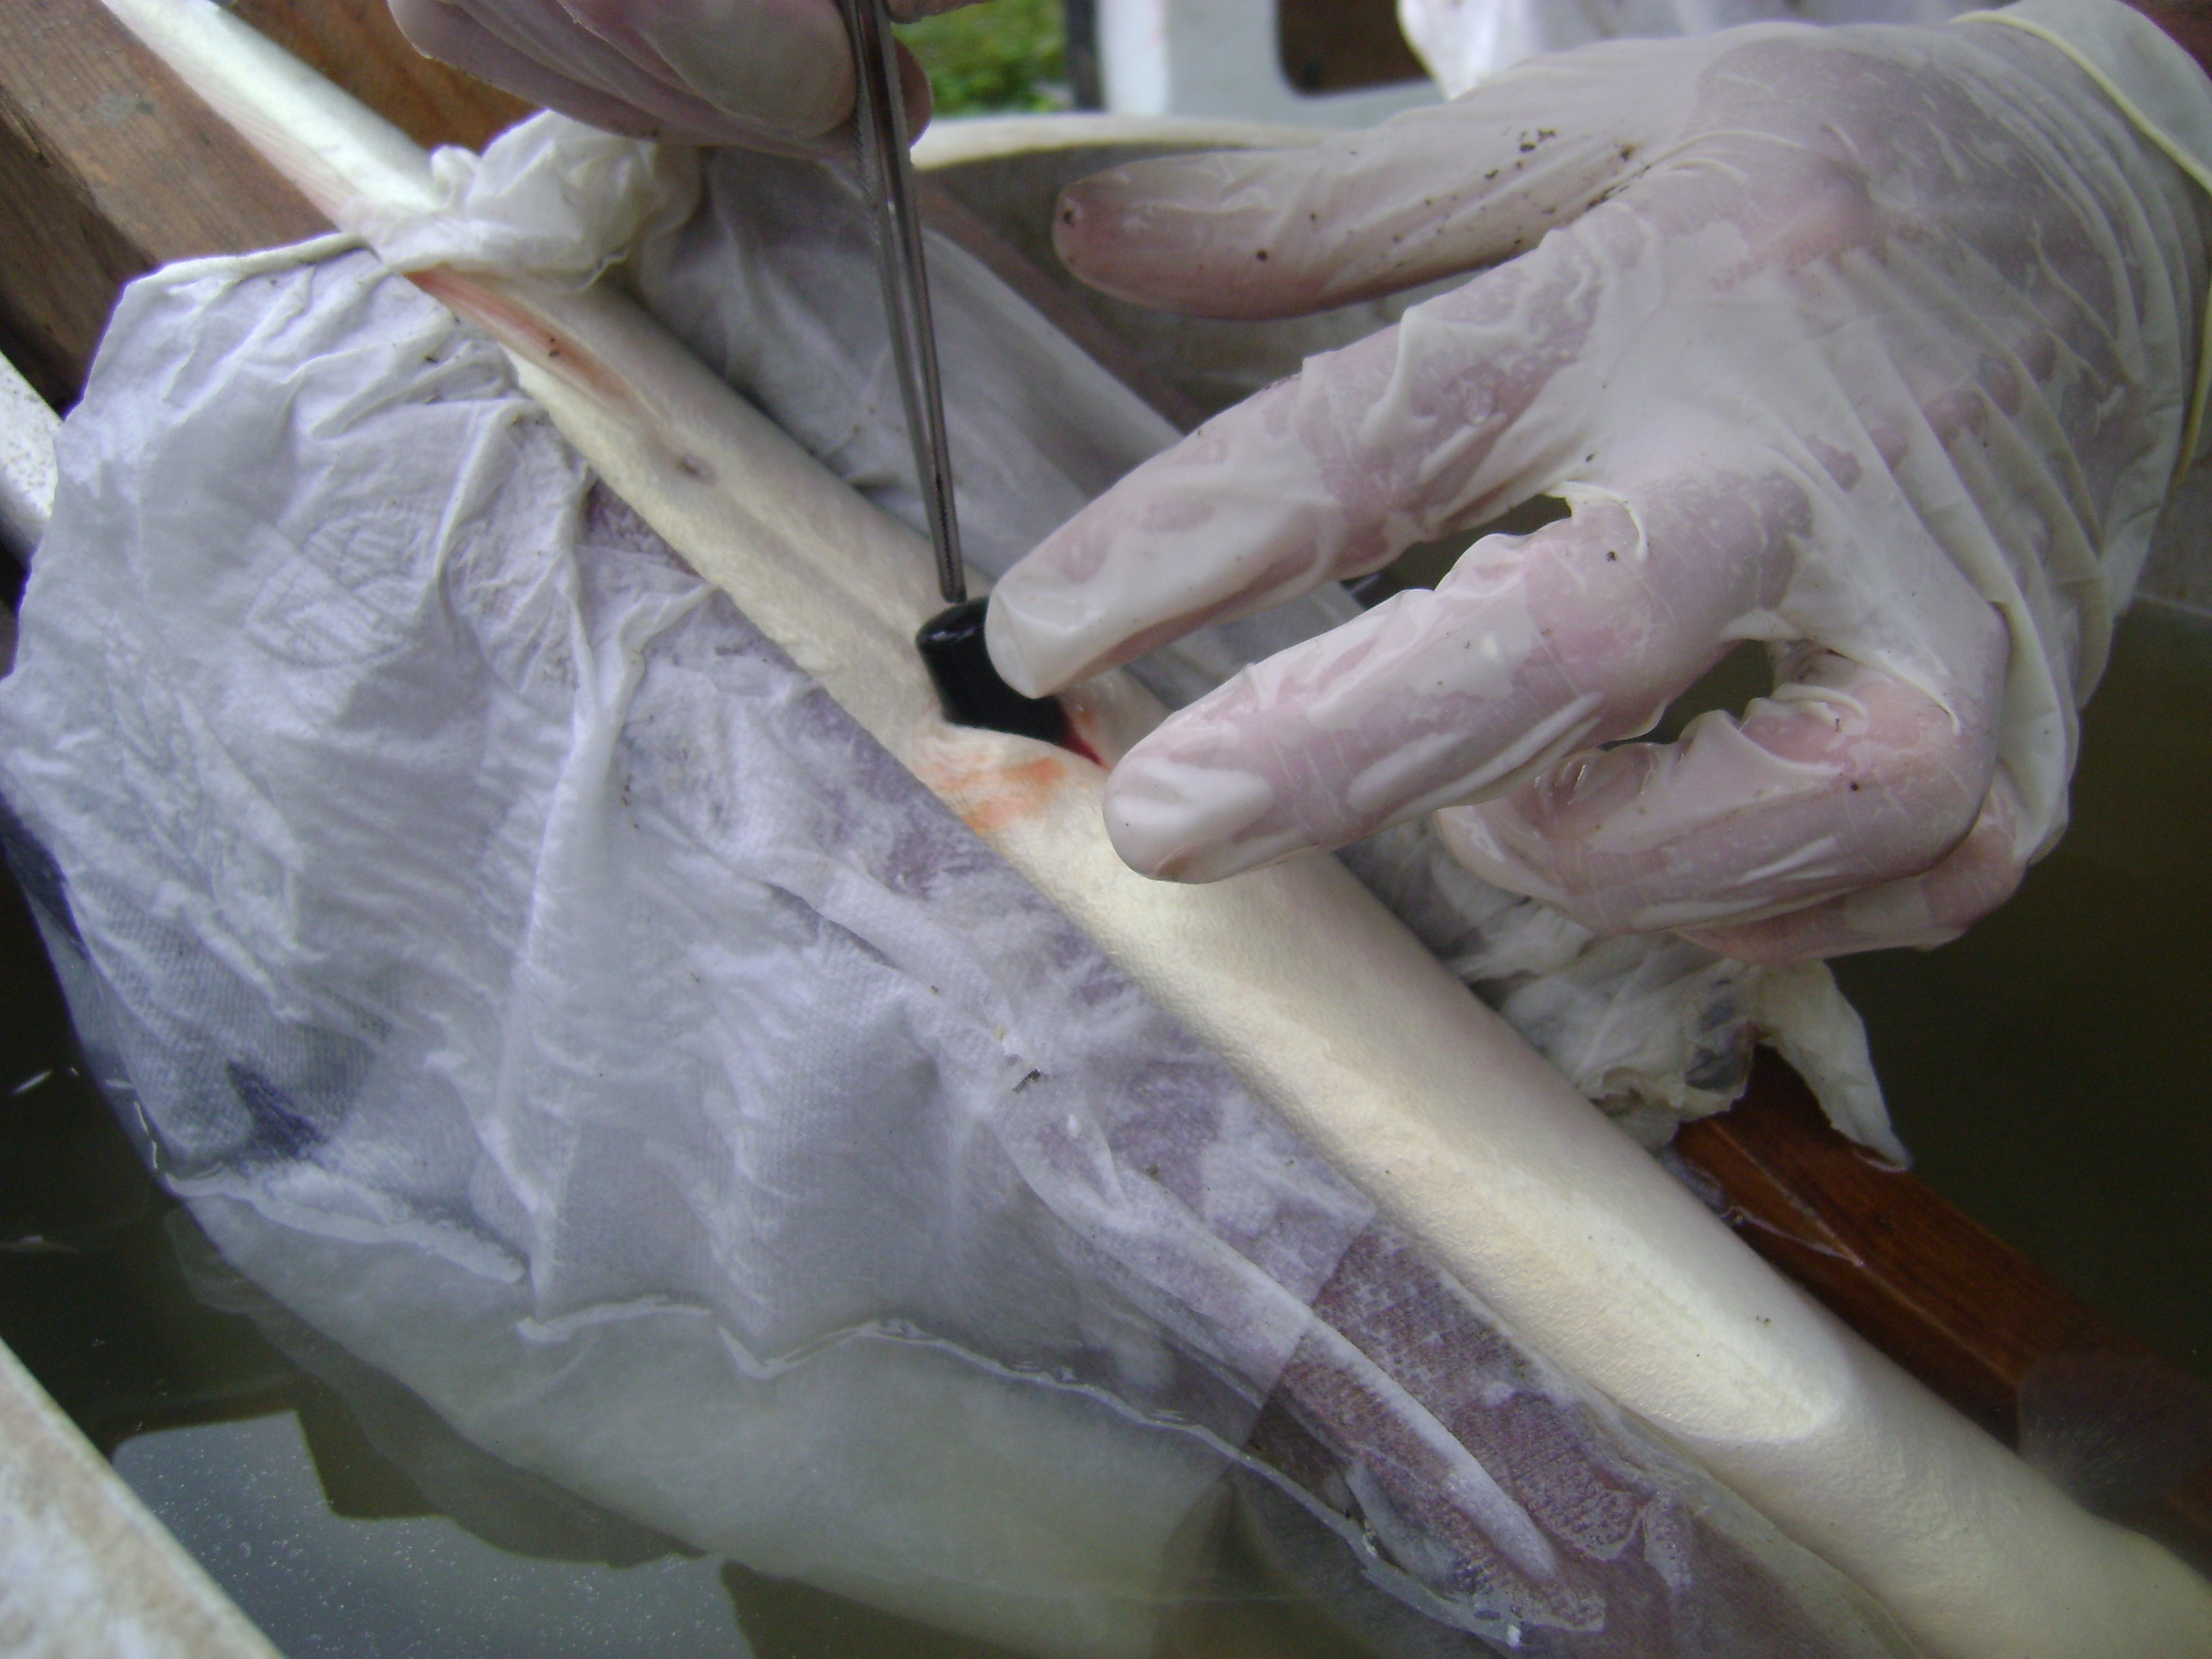
\includegraphics[scale=0.37]{Eeltagged}
  \caption{Internal tagging of eel (\textit{Anguilla anguilla}) with a V13 tag (picture provided by Verhelst P.).}
  \label{fig:Eeltagged}
\end{figure}

\begin{figure}[h!]
  \centering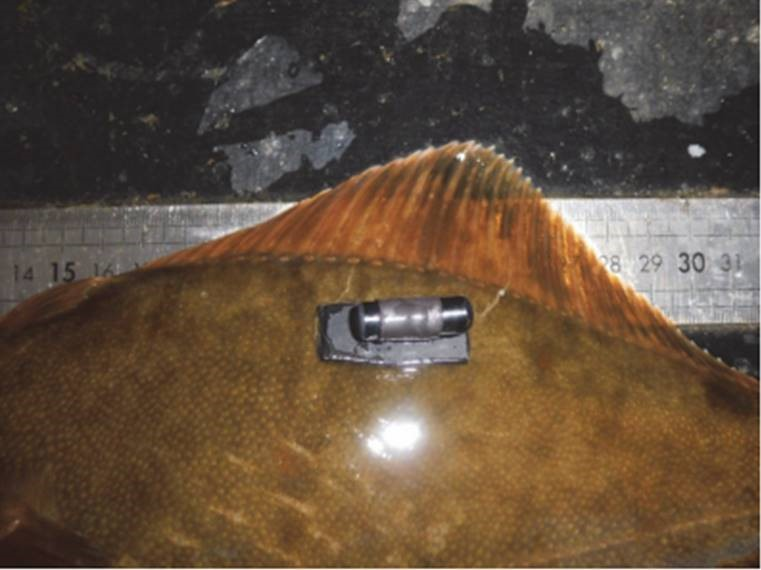
\includegraphics[scale=0.57]{Floundertagged}
  \caption{External tagging of flounder (\textit{Platichthys flesus}) with a V7 tag (picture provided by Verhelst P.).}
  \label{fig:Floundertagged}
\end{figure}

\clearpage

\section{Data processing}
\label{Dataprocessing}
\FloatBarrier

\setcounter{table}{0} \renewcommand{\thetable}{B.\arabic{table}}
\setcounter{figure}{0} \renewcommand{\thefigure}{B.\arabic{figure}}

This practical example describes how detection groups are transformed in residencies-between receivers: Consider a network of three gates \RNum{1}, \RNum{2} and \RNum{3}, spatially aligned as such (Fig. \ref{fig:detectionInterval}). A tagged fish has a detection group \RNum{1}-\RNum{2} with a time lapse of 0.5 hour (type 1A) and another detection group \RNum{1}-\RNum{3} with a time lapse of 1 hour (type 2), which is probably because the fish swam from \RNum{1} to \RNum{2} in 0.5 hours and subsequently circled around \RNum{2} for one hour without being detected at \RNum{1} or \RNum{3}. Hence we know that the residencies-between-receivers are between 0.5 to 1.5 hours in section \RNum{1}-\RNum{2} and 0 to 1 hour in \RNum{2}-\RNum{3}. Since there is no spatial overlap in section \RNum{1}-\RNum{3} the residency-between-receivers can be estimated exactly as 1.5 hour. On the one hand, the gate network resolution of the sections \RNum{1}-\RNum{2} and \RNum{2}-\RNum{3} combined, is higher than the gate network resolution of section \RNum{1}-\RNum{3} alone. On the other hand, the residencies-between-receivers of sections \RNum{1}-\RNum{2} and \RNum{2}-\RNum{3} have a higher epistemic uncertainty than the residency-between-receivers of section \RNum{1}-\RNum{3}, because the range of possible residency-between-receivers values is smaller for the latter. It is expected that if more gates are contained within one section, the epistemic uncertainty of that section will be less. The residencies-between-receivers for all possible combinations of sections for all tagged fish were calculated for the analysis.  

\begin{figure}[h!]
  \centering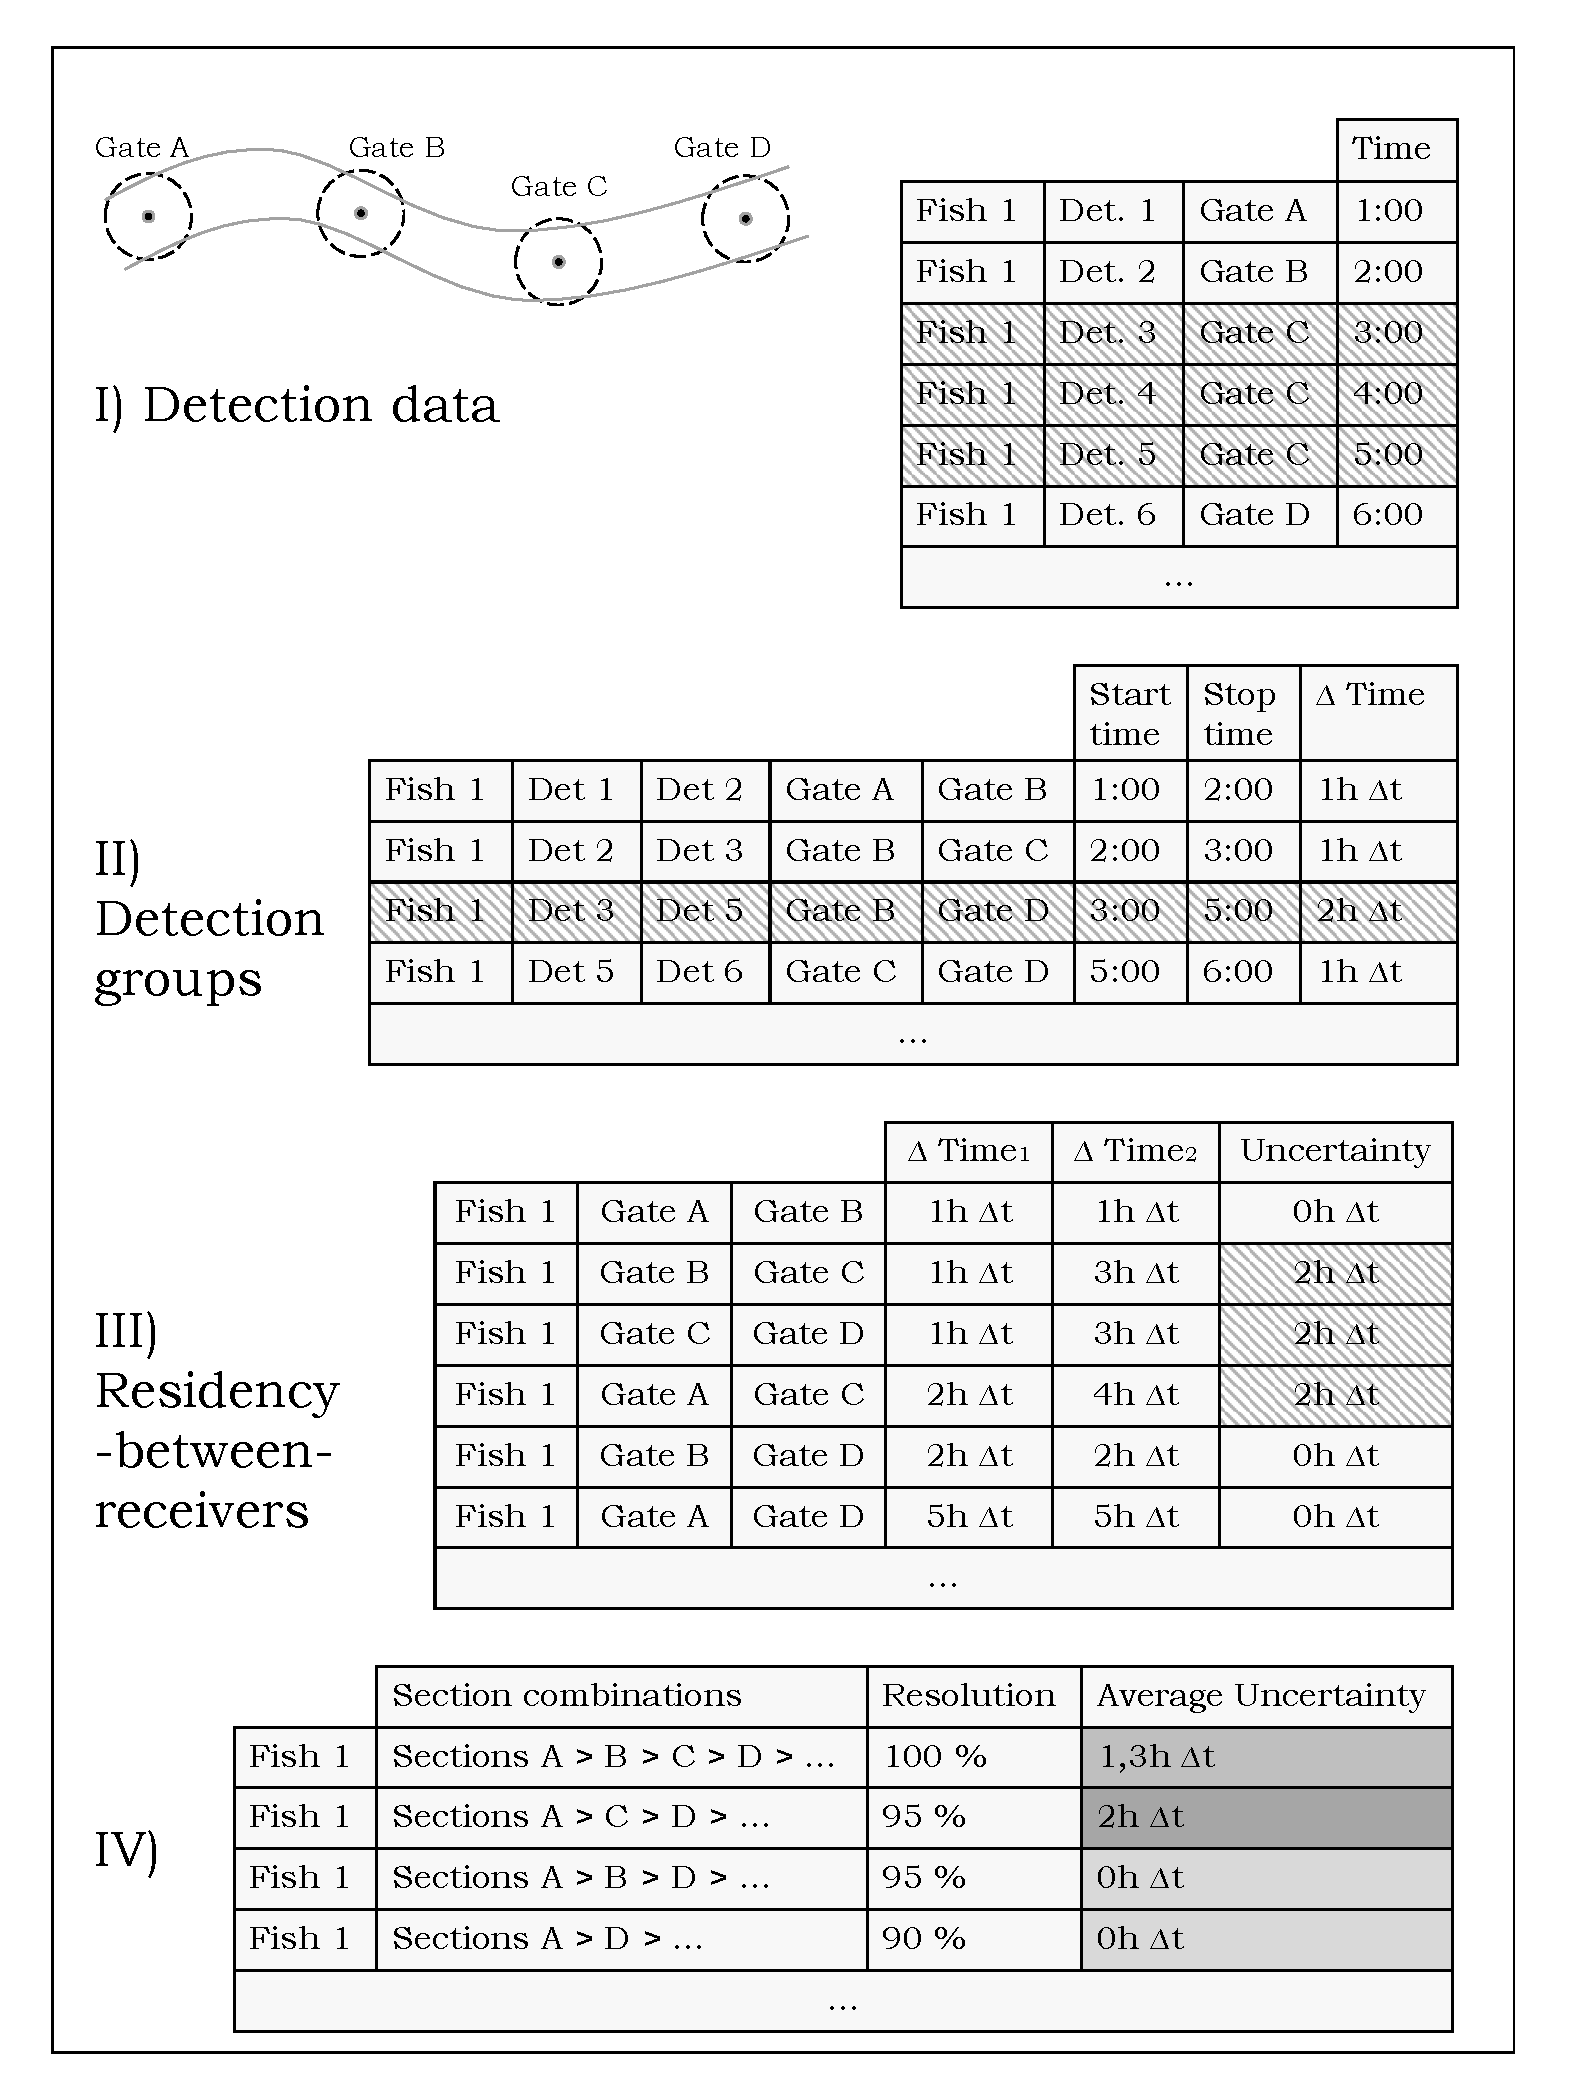
\includegraphics[scale=0.38]{Flow_chart.pdf}
  \caption{Data processing of detection data. I) The shaded detections were all tied up to one specific gate but it is unknown whether the tagged fish resided left or right of the gate during this period. This will introduce some epistemic uncertainty. II) Detections are transformed to detection groups. The shaded detections are combined in one detection group. III) Residencies-between-receivers are estimated from the detection groups. $\bigtriangleup$Time$_{1}$ and $\bigtriangleup$Time$_{2}$ represent the lower and upper bound of the residency-between-receivers intervals respectively. The epistemic uncertainty of the shaded detections is quantified. IV) Section combinations for different gate network resolutions are calculated. For a gate network resolution of 95 \% The section combination A,C,D has a higher average epistemic uncertainty than combination A,B,D. Hence, the latter is retained.}
  \label{fig:Flow_chart}
\end{figure}

\clearpage

\section{Tables}

\setcounter{table}{0} \renewcommand{\thetable}{C.\arabic{table}}
\setcounter{figure}{0} \renewcommand{\thefigure}{C.\arabic{figure}}

\begin{table}[h!]
\centering
\scriptsize
\caption{Detection probability of the entire network (ZS+WS), the Zeeschelde (ZS) section and the Westerschelde (WS) section for tagged eel. Because of the potentially large gaps between the receivers of the gates closer to the sea, assuming that fish were present between these gates may be erroneous. Therefore, we calculated the detection probability for two different scenarios. For scenario 1 we assumed that tagged fish reach the North Sea either way, even when they are not detected at any of the last three gates. For scenario 2 we assumed that tagged fish only reach the North Sea when they are detected at the last gate or at the network of the North Sea. \label{tab:det.prob.cases}}
\begin{tabular}{|l|l|l|l|} 
\hline
\multirow{2}{*}{Scenario} & \multicolumn{3}{l|}{Det. prob. (\% at section ...~ )}  \\ 
\cline{2-4}
                          & ZS+WS & ZS   & WS                                      \\ 
\hline
1                         & 92.3  & 95.8 & 46.4                                    \\ 
\hline
2                         & 95.5  & 97.0 & 62.5                                    \\
\hline
\end{tabular}
\end{table}

\begin{table}
\centering
\scriptsize
\caption{List of gates, with distance from Ghent (km), deployment date, number of included receivers, period of receiver inactivity and detection probability. Receiver inactivity represents the period during which one receiver of the gate was inactive. For example, four receivers of Gate ws2 were inactive during four different periods, which are given in the table.}
\label{gate list}
\begin{tabular}{|c|c|c|c|c|c|} 
\hline
\begin{tabular}[c]{@{}c@{}}gate\\name \end{tabular} & \begin{tabular}[c]{@{}c@{}}Distance\\(km) \end{tabular} & \begin{tabular}[c]{@{}c@{}}Deployment\\date \end{tabular} & \begin{tabular}[c]{@{}c@{}}number\\of receivers \end{tabular} & receiver inactivity          & \begin{tabular}[c]{@{}c@{}}Det. prob. (\%\\eel (flounder)\end{tabular}  \\ 
\hline
s1                                                  & 0.0                                                     & 31/03/2015                                                & 1                                                       &                         & 100.0                                                                   \\ 
\hline
s2                                                  & 6.6                                                     & 20/03/2016                                                & 1                                                       &                         & 100.0                                                                   \\ 
\hline
s3                                                  & 12.1                                                    & 20/03/2016                                                & 1                                                       &                         & 97.1                                                                    \\ 
\hline
s4                                                  & 16.8                                                    & 20/04/2015                                                & 1                                                       &                         & 97.4                                                                    \\ 
\hline
s5                                                  & 26.7                                                    & 31/03/2015                                                & 1                                                       &                         & 99.1                                                                    \\ 
\hline
s6                                                  & 30.6                                                    & 2/04/2015                                                 & 1                                                       &                         & 98.7                                                                    \\ 
\hline
s7                                                  & 33.0                                                    & 24/03/2016                                                & 1                                                       & 17/10/2017 - 24/11/2017 & 96.7                                                                    \\ 
\hline
s8                                                  & 39.3                                                    & 24/03/2016                                                & 1                                                       &                         & 81.6                                                                    \\ 
\hline
s9                                                  & 40.8                                                    & 20/04/2015                                                & 1                                                       &                         & 99.9                                                                    \\ 
\hline
s10                                                 & 44.1                                                    & 20/04/2015                                                & 1                                                       &                         & 99.3                                                                    \\ 
\hline
s11                                                 & 46.5                                                    & 27/04/2015                                                & 1                                                       &                         & 100.0                                                                   \\ 
\hline
s12                                                 & 49.0                                                    & 2/04/2015                                                 & 1                                                       &                         & 98.4                                                                    \\ 
\hline
s13                                                 & 53.8                                                    & 2/04/2015                                                 & 1                                                       &                         & 93.2                                                                    \\ 
\hline
s14                                                 & 55.6                                                    & 2/04/2015                                                 & 1                                                       &                         & 100.0                                                                   \\ 
\hline
s15                                                 & 63.3                                                    & 2/04/2015                                                 & 2                                                       &                         & 100.0 (87.5)                                                            \\ 
\hline
s16                                                 & 68.6                                                    & 2/04/2015                                                 & 2                                                       &                         & 100.0 (66.7)                                                            \\ 
\hline
s17                                                 & 75.8                                                    & 30/09/2015                                                & 3                                                       &                         & 100.0 (0)                                                               \\ 
\hline
s18                                                 & 88.2                                                    & 3/09/2015                                                 & 2                                                       &                         & 77.8 (50.0)                                                             \\ 
\hline
ws1                                                 & 112.8                                                   & 22/09/2015                                                & 6                                                       &                         & 91.3 (50.0)                                                             \\ 
\hline
ws2                                                 & 135.1                                                   & 1/07/2012                                                 & 21                                                      & 1/7/2012 - 29/12/2014   & 45.2 (33.3)                                                             \\ 
\cline{5-5}
                                                    &                                                         &                                                           &                                                         & 30/12/2014 - 22/2/2015  &                                                                         \\ 
\cline{5-5}
                                                    &                                                         &                                                           &                                                         & 15/10/2014 - 10/2/2015  &                                                                         \\ 
\cline{5-5}
                                                    &                                                         &                                                           &                                                         & 30/1/2014 - 11/2/2015   &                                                                         \\ 
\hline
ws3                                                 & 154.5                                                   & 22/05/2014                                                & 12                                                      & 15/1/2015 - 19/3/2015   & 29.2                                                                    \\ 
\cline{5-5}
                                                    &                                                         &                                                           &                                                         & 8/5/2015 - 9/9/2015     &                                                                         \\
\hline
\end{tabular}
\end{table}

\begin{table}
\centering
\scriptsize
\caption{List of tagged eels, with last station detected, detection probability, and tag power output (PO; L = low power output, H = high power output).}
\label{tag_list}
\begin{tabular}{|c|c|c|c|} 
\hline
Eel tag code            & Last station detected & Det. prob. (\%) & PO  \\ 
\hline
A69-1601-52623 & ws3                   & 100.0                & H   \\ 
\hline
A69-1601-52625 & ws3                   & 100.0                & H   \\ 
\hline
A69-1601-52635 & ws3                   & 100.0               & H   \\ 
\hline
A69-1601-52645 & ws3                   & 100.0                & H   \\ 
\hline
A69-1601-52649 & ws3                   & 100.0                & H   \\ 
\hline
A69-1601-52632 & ws3                   & 97.0                 & H   \\ 
\hline
A69-1601-52662 & ws3                   & 95.7                 & H   \\ 
\hline
A69-1602-30330 & ws2                   & 95.5                 & H   \\ 
\hline
A69-1602-30333 & ws3                   & 95.2                 & H   \\ 
\hline
A69-1601-52642 & ws2                   & 95.0                 & H   \\ 
\hline
A69-1601-52622 & ws3                   & 94.7                 & H   \\ 
\hline
A69-1601-52629 & ws3                   & 94.7                 & H   \\ 
\hline
A69-1601-52633 & ws3                   & 94.7                 & H   \\ 
\hline
A69-1601-52636 & ws3                   & 94.7                 & H   \\ 
\hline
A69-1601-52647 & ws3                   & 94.7                 & H   \\ 
\hline
A69-1601-52654 & ws3                   & 94.7                 & H   \\ 
\hline
A69-1602-30346 & ws3                   & 94.7                 & H   \\ 
\hline
A69-1601-57472 & ws2                   & 93.8                 & L   \\ 
\hline
A69-1602-30352 & ws1                   & 92.9                 & H   \\ 
\hline
A69-1601-52644 & ws3                   & 91.2                 & H   \\ 
\hline
A69-1601-52639 & ws1                   & 90.9                 & H   \\ 
\hline
A69-1602-30332 & ws1                   & 90.9                 & H   \\ 
\hline
A69-1602-30331 & ws3                   & 90.9                 & H   \\ 
\hline
A69-1602-30337 & ws2                   & 90.5                 & H   \\ 
\hline
A69-1601-52653 & ws1                   & 90.0                 & H   \\ 
\hline
A69-1602-30343 & ws1                   & 90.0                & H   \\ 
\hline
A69-1602-30345 & ws1                   & 90.0                & H   \\ 
\hline
A69-1602-30355 & ws1                   & 90.0                & H   \\ 
\hline
A69-1602-30344 & ws3                   & 90.0                 & H   \\ 
\hline
A69-1601-52641 & ws2                   & 89.5                 & H   \\ 
\hline
A69-1601-52648 & ws2                   & 89.5                 & H   \\ 
\hline
A69-1601-52651 & ws2                   & 89.5                 & H   \\ 
\hline
A69-1602-30356 & ws1                   & 88.9                 & H   \\ 
\hline
A69-1601-52664 & ws3                   & 88.9                 & H   \\ 
\hline
A69-1602-30350 & ws3                   & 88.9                & H   \\ 
\hline
A69-1601-52638 & s18                   & 85.0                 & H   \\ 
\hline
A69-1601-57475 & ws3                   & 85.0                 & L   \\ 
\hline
A69-1601-57470 & ws1                   & 80.0                 & L   \\
\hline
\end{tabular}
\end{table}

\begin{table}
\centering
\scriptsize
\caption{Output of the fixed effects of the linear mixed effects model with log-transformed epistemic uncertainty as response, gate network resolution and removed station as fixed effect and eel as random effect. The values, standard errors (SE), degrees of freedom (DF), t-values and p-values are given. The p-values of the post-hoc tests of the factor removed station were corrected using the Bonferroni approach. Only comparisons resulting in significant p-values are given. For the original combinations of sections bordered by gates no gates were omitted.}
\label{lmer model stations removed}
\resizebox{\columnwidth-235pt}{!}{%
\begin{tabular}{|l|l|l|l|l|l|}
\hline
Coefficient & SE   & DF    & t-value & p-value & Effect       \\ \hline
0.11        & 0.00 & 12742 & 406.02  & 0.00    & resolution   \\ \hline
-11.50      & 0.14 & 12742 & -84.32  & 0.00    & intercept    \\ \hline
0.40        & 0.04 & 12742 & 10.48   & 0.00    & original-ws2 \\ \hline
0.39        & 0.04 & 12742 & 10.15   & 0.00    & original-ws1 \\ \hline
0.32        & 0.04 & 12742 & 8.35    & 0.00    & original-s4  \\ \hline
0.31        & 0.04 & 12742 & 8.23    & 0.00    & original-s12 \\ \hline
0.31        & 0.04 & 12742 & 8.20    & 0.00    & original-s2  \\ \hline
0.31        & 0.04 & 12742 & 8.03    & 0.00    & originals-18 \\ \hline
0.30        & 0.04 & 12742 & 7.95    & 0.00    & original-s17 \\ \hline
0.26        & 0.04 & 12742 & 6.86    & 0.00    & original-s15 \\ \hline
0.26        & 0.04 & 12742 & 6.81    & 0.00    & original-s9  \\ \hline
0.25        & 0.04 & 12742 & 6.64    & 0.00    & original-s8  \\ \hline
0.25        & 0.04 & 12742 & 6.49    & 0.00    & s10-ws2      \\ \hline
0.25        & 0.04 & 12742 & 6.34    & 0.00    & s11-ws2      \\ \hline
0.24        & 0.04 & 12742 & 6.29    & 0.00    & original-s16 \\ \hline
0.24        & 0.04 & 12742 & 6.28    & 0.00    & original-s7  \\ \hline
0.24        & 0.04 & 12742 & 6.16    & 0.00    & s10-ws1      \\ \hline
0.23        & 0.04 & 12742 & 6.00    & 0.00    & s11-ws1      \\ \hline
0.22        & 0.04 & 12742 & 5.63    & 0.00    & s14-ws2      \\ \hline
0.22        & 0.04 & 12742 & 5.58    & 0.00    & s6-ws2       \\ \hline
0.21        & 0.04 & 12742 & 5.56    & 0.00    & original-s3  \\ \hline
0.21        & 0.04 & 12742 & 5.52    & 0.00    & original-s5  \\ \hline
0.21        & 0.04 & 12742 & 5.41    & 0.00    & s13-ws2      \\ \hline
0.20        & 0.04 & 12742 & 5.30    & 0.00    & s14-ws1      \\ \hline
0.20        & 0.04 & 12742 & 5.25    & 0.00    & s6-ws1       \\ \hline
0.20        & 0.04 & 12742 & 5.07    & 0.00    & s13-ws1      \\ \hline
0.19        & 0.04 & 12742 & 5.02    & 0.00    & original-s13 \\ \hline
0.19        & 0.04 & 12742 & 4.90    & 0.00    & s5-ws2       \\ \hline
0.19        & 0.04 & 12742 & 4.86    & 0.00    & s3-ws2       \\ \hline
0.18        & 0.04 & 12742 & 4.83    & 0.00    & original-s6  \\ \hline
0.18        & 0.04 & 12742 & 4.79    & 0.00    & original-s14 \\ \hline
0.18        & 0.04 & 12742 & 4.56    & 0.00    & s5-ws1       \\ \hline
0.18        & 0.04 & 12742 & 4.53    & 0.00    & s3-ws1       \\ \hline
0.17        & 0.04 & 12742 & 4.38    & 0.00    & s10-s4       \\ \hline
0.16        & 0.04 & 12742 & 4.25    & 0.00    & s10-s12      \\ \hline
0.16        & 0.04 & 12742 & 4.23    & 0.00    & s10-s2       \\ \hline
0.16        & 0.04 & 12742 & 4.22    & 0.00    & s11-s4       \\ \hline
0.16        & 0.04 & 12742 & 4.15    & 0.01    & s7-ws2       \\ \hline
0.16        & 0.04 & 12742 & 4.14    & 0.01    & s16-ws2      \\ \hline
0.16        & 0.04 & 12742 & 4.09    & 0.01    & s11-s12      \\ \hline
0.16        & 0.04 & 12742 & 4.08    & 0.01    & s11-s2       \\ \hline
0.16        & 0.04 & 12742 & 4.06    & 0.01    & s10-s18      \\ \hline
0.15        & 0.04 & 12742 & 4.06    & 0.01    & original-s11 \\ \hline
0.15        & 0.04 & 12742 & 3.99    & 0.01    & s10-s17      \\ \hline
0.15        & 0.04 & 12742 & 3.91    & 0.02    & s11-s18      \\ \hline
0.15        & 0.04 & 12742 & 3.90    & 0.02    & original-s10 \\ \hline
0.15        & 0.04 & 12742 & 3.83    & 0.02    & s11-s17      \\ \hline
0.15        & 0.04 & 12742 & 3.84    & 0.02    & s8-ws2       \\ \hline
0.15        & 0.04 & 12742 & 3.81    & 0.03    & s7-ws1       \\ \hline
0.15        & 0.04 & 12742 & 3.81    & 0.03    & s16-ws1      \\ \hline
\end{tabular}
}
\end{table}

\FloatBarrier

\section{Figures}

\setcounter{table}{0} \renewcommand{\thetable}{D.\arabic{table}}
\setcounter{figure}{0} \renewcommand{\thefigure}{D.\arabic{figure}}

\begin{figure}[h!]
  \centering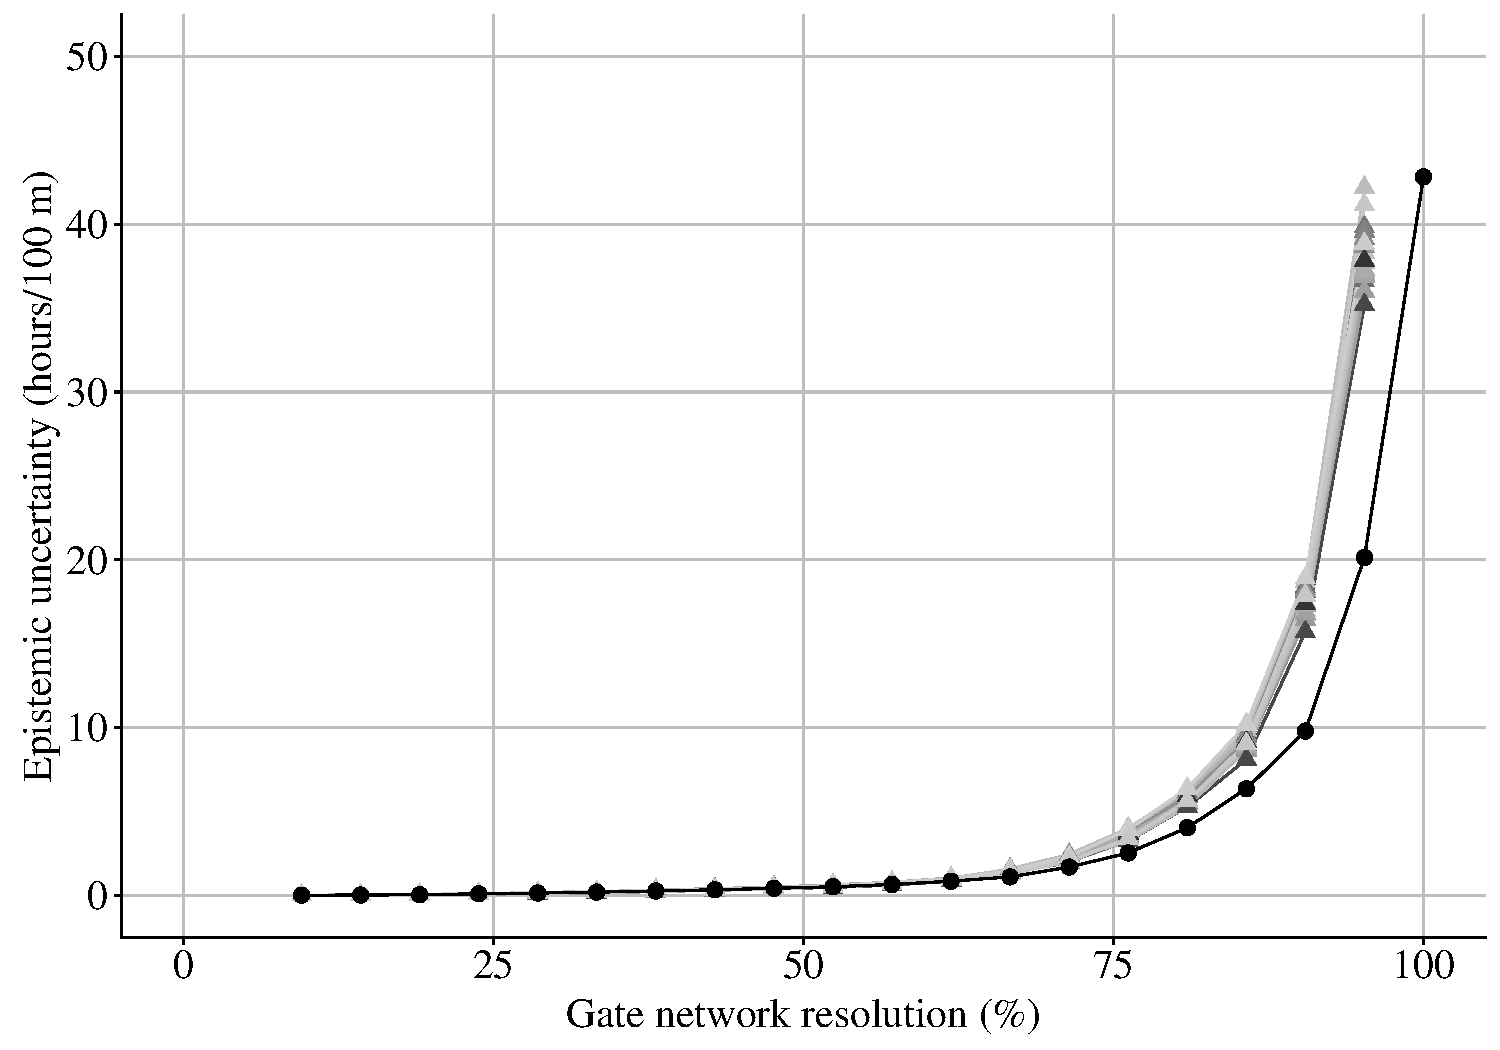
\includegraphics[scale=0.45]{Pareto_stations_removed_duration.pdf}
  \caption{Effect of omitting specific gates on trade-off between epistemic uncertainty (vertical axis) and gate network resolution (horizontal axis). The average trade-off of all 38 eels was calculated. Each curve with triangle dots represents different section combination trade-offs with different gates being omitted. The black curve with the circle dots represents the original trade-off without any gates being omitted.}
  \label{fig:Pareto_stations_removed}
\end{figure}

\begin{figure}[h!]
  \centering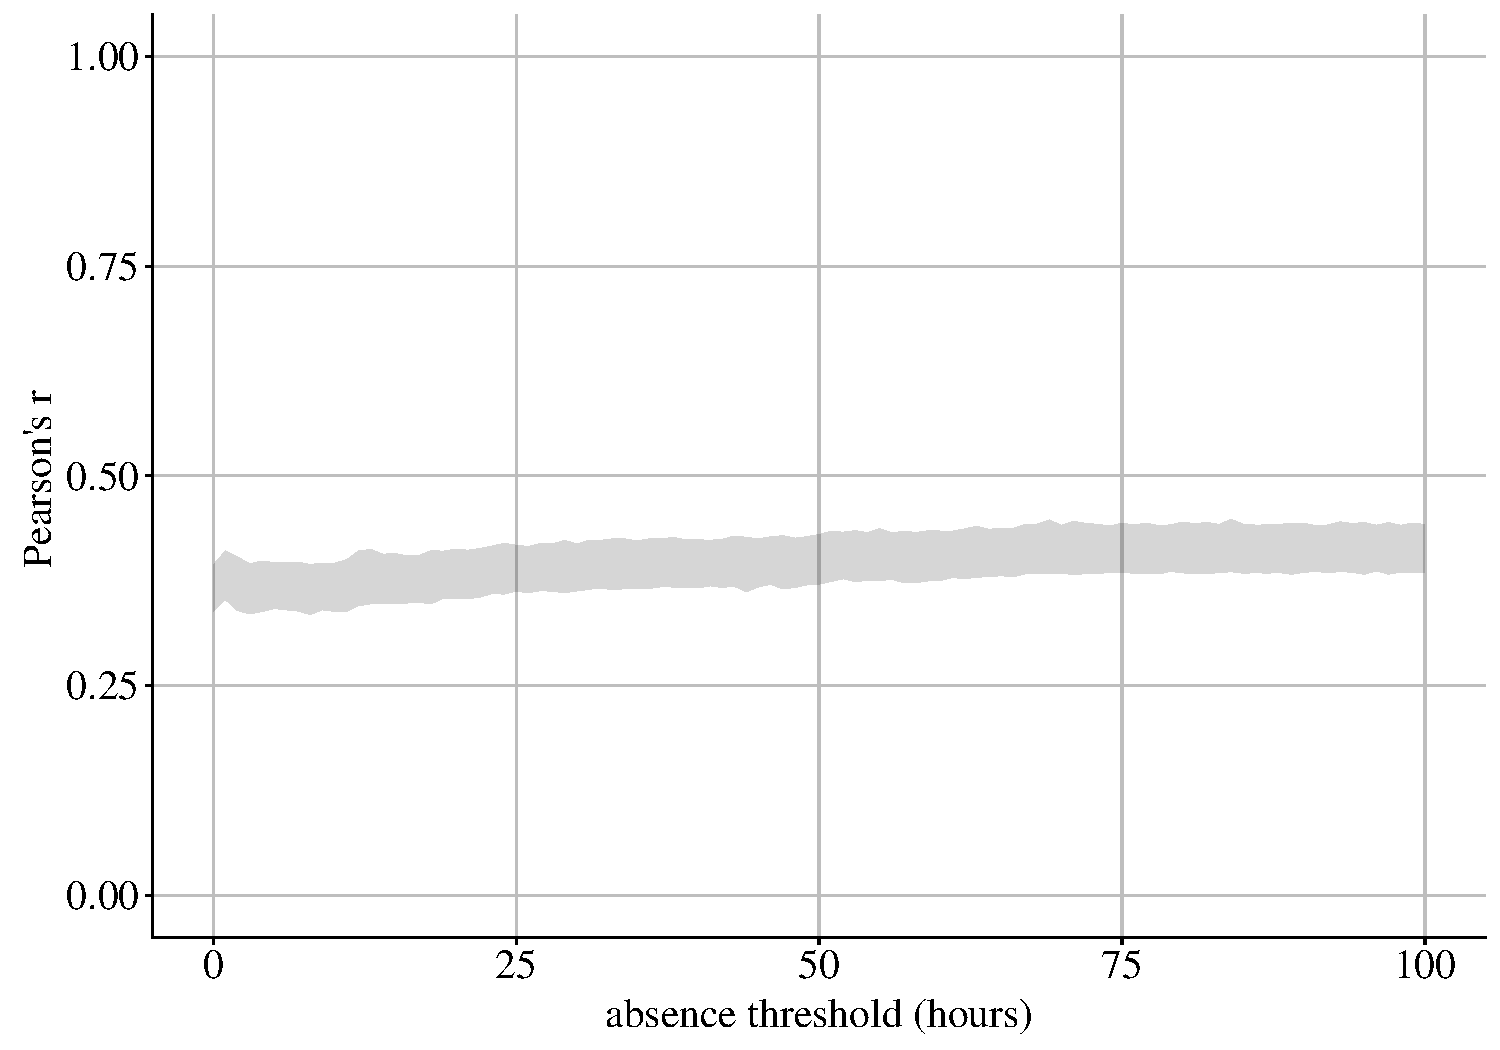
\includegraphics[scale=0.45]{correlation_activity_and_gate_period.pdf}
  \caption{Pearson's correlation coefficient ($r$) of residencies-between-receivers and residencies-at-receivers for different absence threshold values. Monte Carlo simulations (10$^{6}$) were used to determine the band of possible $r$ values.}
  \label{fig:correlation}
\end{figure}

\begin{figure}[h!]
  \centering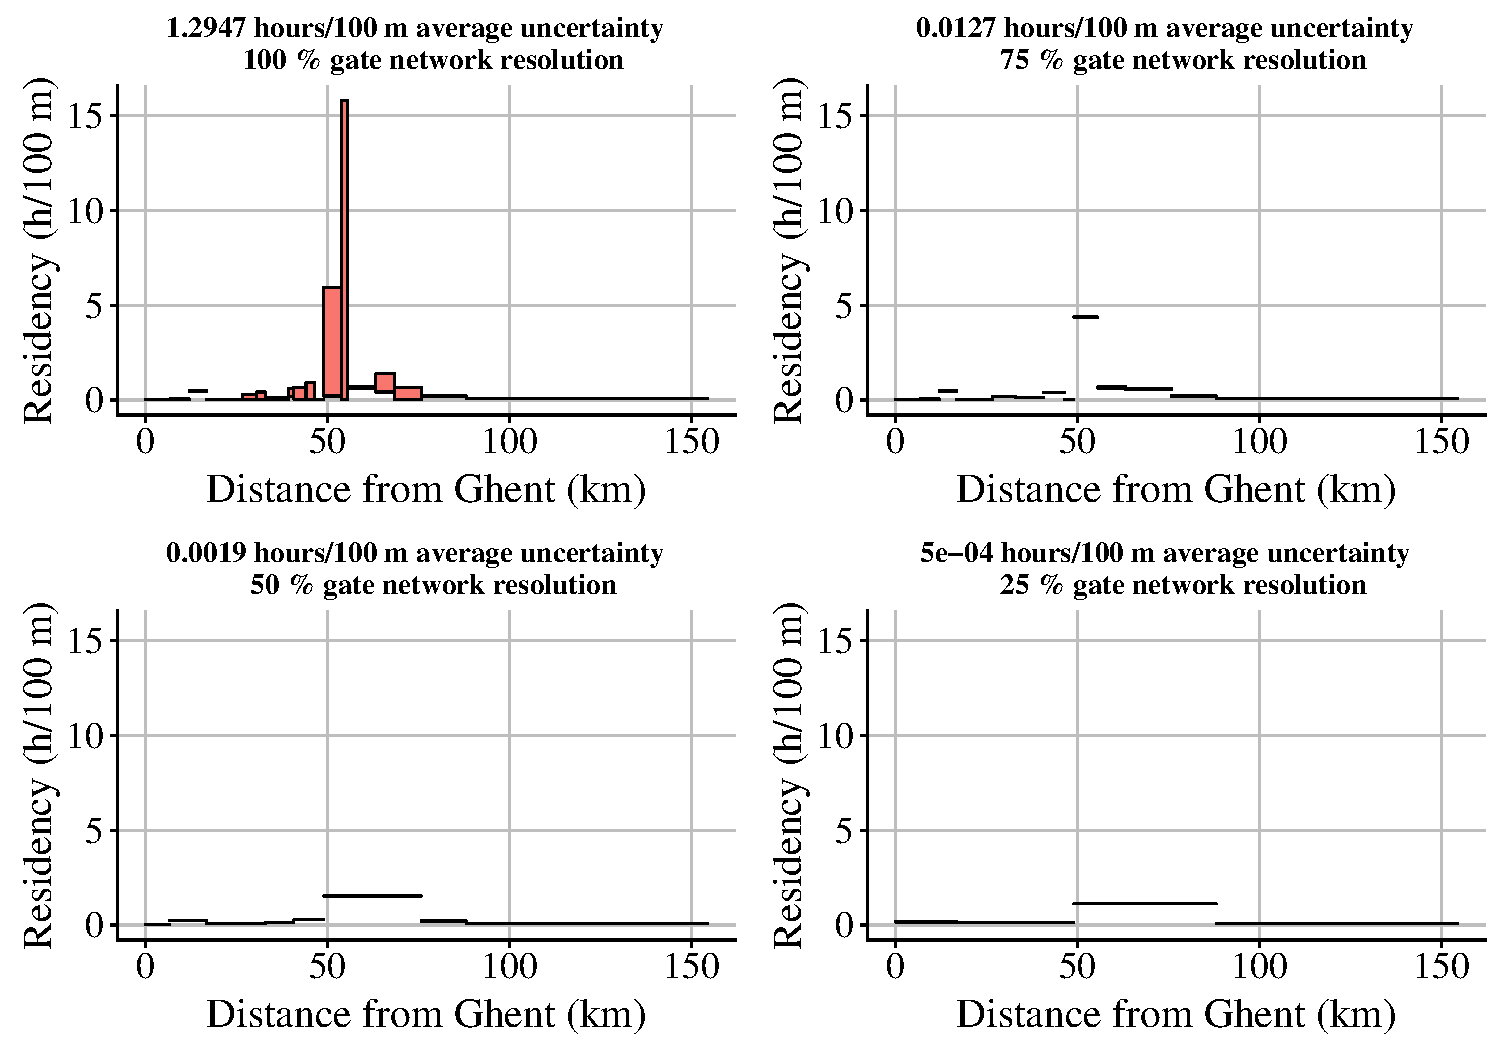
\includegraphics[scale=0.45]{Resistance_model2_jb_eel2.pdf}
  \caption{Residency-between-receivers (hours/100m) in function of distance from Ghent (km). Combinations of sections bordered by gates for eel "A69-1601-52623" with different levels of gate network resolution and different levels of average epistemic uncertainty are depicted. The range between the minimum and maximum value of the residencies-between-receivers, i.e. the epistemic uncertainty, is represented by the red boxes.}
  \label{fig:Resistance_model2}
\end{figure}

\begin{figure}[h!]
  \centering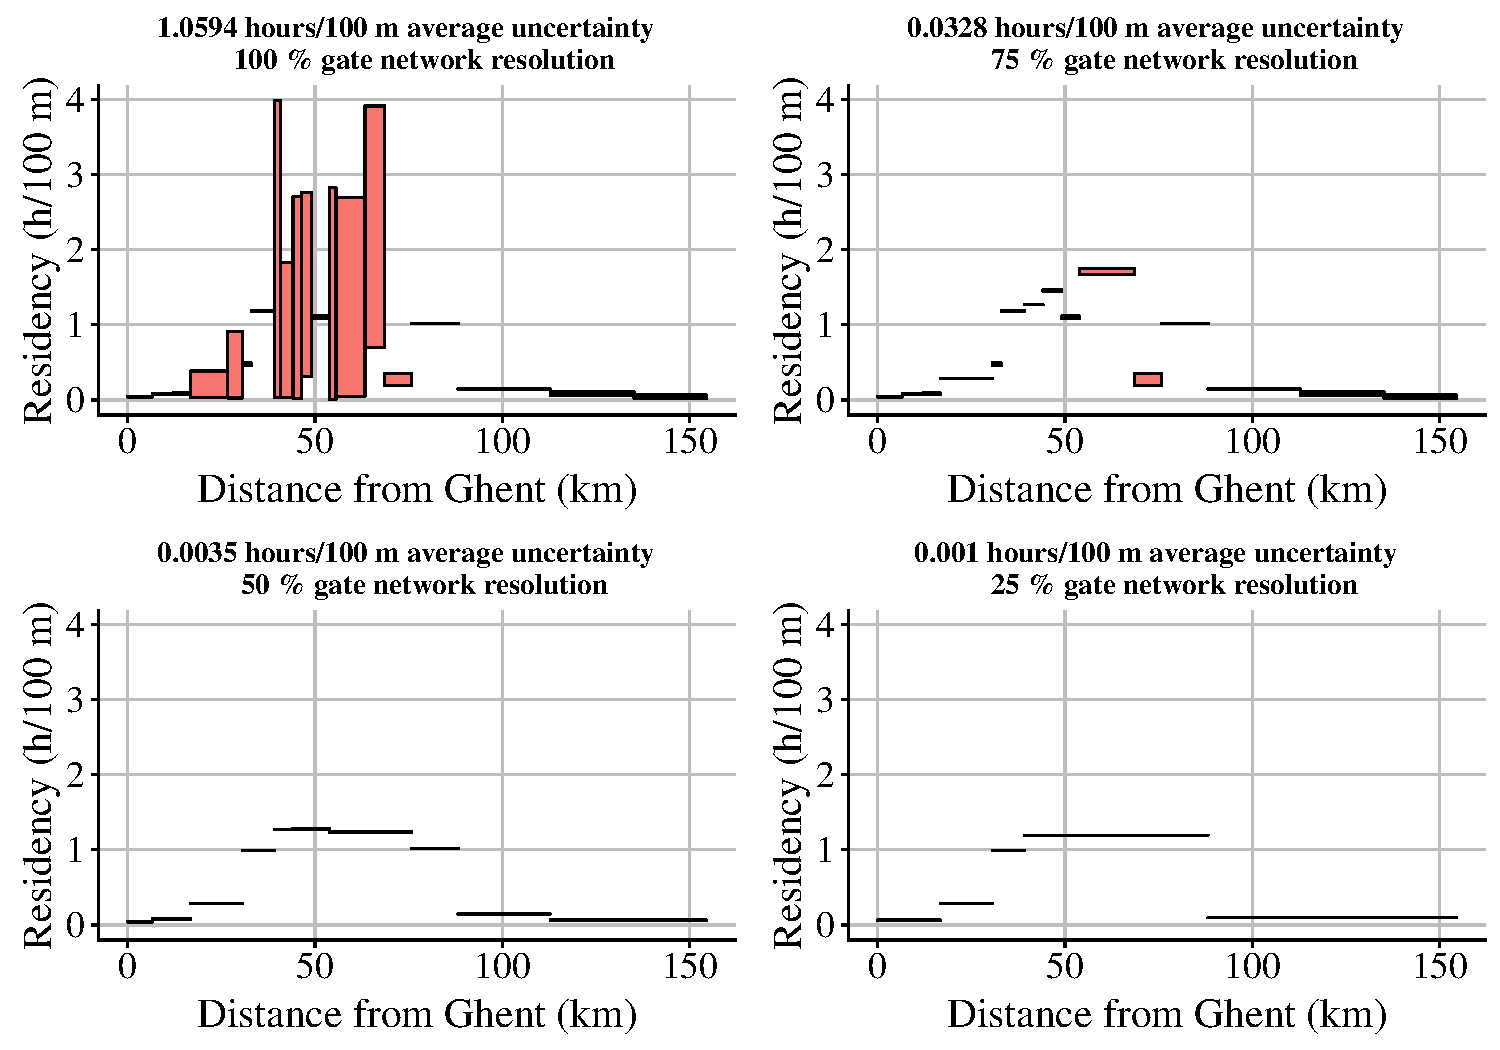
\includegraphics[scale=0.45]{Resistance_model2_jb_eel3.pdf}
  \caption{Residency-between-receivers (hours/100m) in function of distance from Ghent (km). Combinations of sections bordered by gates for eel "A69-1601-52625" with different levels of gate network resolution and different levels of average epistemic uncertainty are depicted. The range between the minimum and maximum value of the residencies-between-receivers, i.e. the epistemic uncertainty, is represented by the red boxes.}
  \label{fig:Resistance_model3}
\end{figure}

\FloatBarrier

\section{Population assessment}
\label{Fig}

\setcounter{table}{0} \renewcommand{\thetable}{E.\arabic{table}}
\setcounter{figure}{0} \renewcommand{\thefigure}{E.\arabic{figure}}

Different tagged eels have different optimal combinations of sections bordered by gates for a specific gate network resolution. For different resolutions, different sections are combined to obtain an optimal reduction in epistemic uncertainty. It is possible to assign each section between gates a midpoint value of the corresponding residency-between-receivers interval, but it should be noted that with decreasing gate network resolution the results are smoothed and spatial information gets lost. A high gate network resolution on the other hand, has the advantage of providing a unique estimate for many different sections, but generally the unaccounted uncertainty of these sections will be high. In Fig. \ref{fig:overall_uncertainty} can be seen that at a gate network resolution of 100 \%, the high level of epistemic uncertainty obscures any potential trend, while at a gate network resolution of 25 \% the extensive loss of spatial information smoothes any potential trend away. It seems that for this case, a gate network resolution of 50 \% allows to detect a simple trend in the duration that eels spend between the different sections.  

\begin{figure}[h!]
  \centering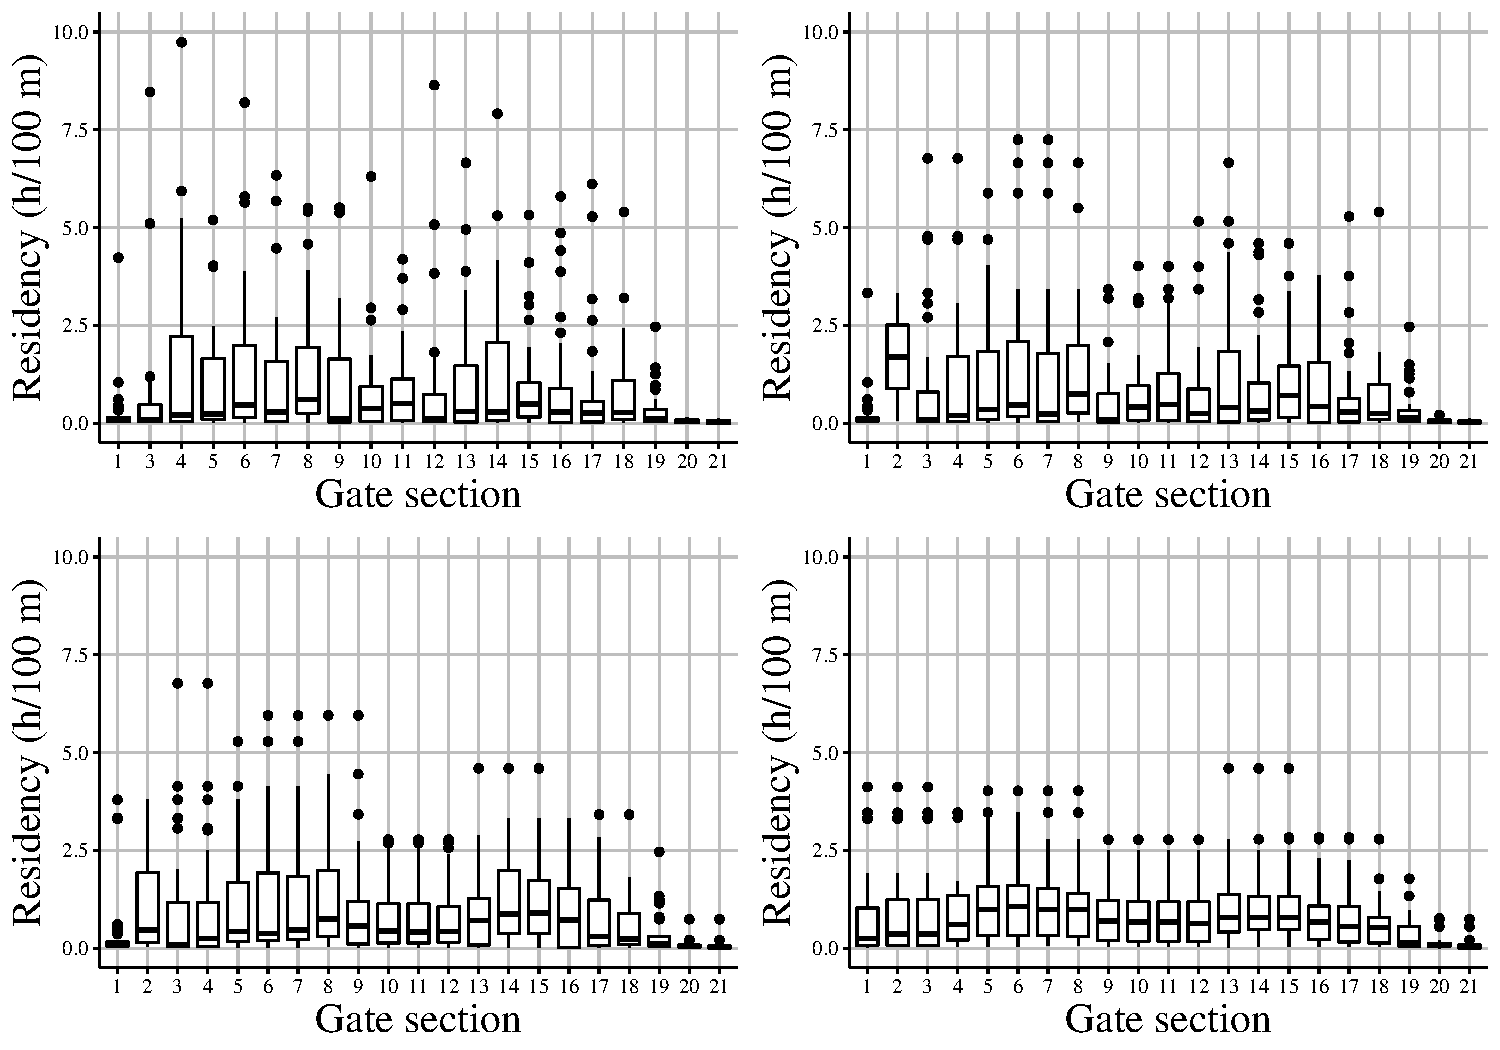
\includegraphics[scale=0.45]{overall_uncertainty.pdf}
  \caption{Boxplots of midpoint values of all residency-between-receivers intervals of all tagged eels.}
  \label{fig:overall_uncertainty}
\end{figure}

\end{spacing}
\end{document}
